
%
%  $Description: Author guidelines and sample document in LaTeX 2.09$ 
%
%  $Author: ienne $
%  $Date: 1995/09/15 15:20:59 $
%  $Revision: 1.4 $
%

\documentclass[times, 10pt,twocolumn]{article} 
\usepackage{amsmath}
\usepackage{latex8}
\usepackage{algorithmic}
\usepackage{algorithm}
\usepackage{amsfonts}
\usepackage{subfigure}
%\usepackage{subfig}
\usepackage{amssymb}
\usepackage[small]{caption}
 \usepackage{graphicx}
\usepackage{amsmath}
\usepackage{multirow}
\usepackage{comment}
\usepackage{enumerate}
\usepackage{latexsym}
\usepackage{tipa}

\usepackage{times}
\newcommand{\bs}[0]{\textrm{\textbackslash}}

\DeclareMathOperator*{\unif}{Unif}

%\documentstyle[times,art10,twocolumn,latex8]{article}

%------------------------------------------------------------------------- 
% take the % away on next line to produce the final camera-ready version 
\pagestyle{empty}

%------------------------------------------------------------------------- 
\begin{document}

\title{An Investigation into Concurrent Expectation Propagation}

\author{David Hall and Alex Kantchelian \\
EECS CS Division \\ University of California, Berkeley\\ \texttt{\{dlwh,
akant\}@cs.berkeley.edu}\\
}

\maketitle
\thispagestyle{empty}

\begin{abstract}
As statistical machine learning becomes more and more prevalent and models become more complicated and fit to larger amounts of data, approximate inference mechanisms become more and more crucial to their success. Expectation propagation (EP) is one such algorithm for inference in probabilistic graphical models. In this work, we introduce a robustified version of EP which helps ensure convergence under a relaxed memory consistency model. The resulting algorithm can be efficiently implemented on a GPU in a straightforward way. Using a 2D Ising spin glass model, we evaluate both the original EP algorithm and our robustified version in terms of convergence, if any, and precision on a classic single core processor. We also compare the naive parallelized version of the original EP algorithm against the parallelized robustified EP on both a multicore CPU and a GPU.
\end{abstract}



\section{Introduction}

\ldots
EP updates are typically defined sequentially,
and there is reason to believe this is intentional.
While some (XXX) have employed parallel updates when using EP, they
have done so uncritically, finding that it works. Here, we
undertake to explore
\ldots

This paper is organized as follows. First, we describe necessary
background on probabilistic graphical models. Second, we describe
different inference algorithms in general and Expectation Propagation
in particular. Third, we motivate and present Convex Expectation
Propagation. Finally, we conduct our experiments on synthetic
models in a Ising spin-glass model under a variety of parameter
conditions.

\section{Graphical Models}

\begin{figure}
  [ising model here XXX]
  \caption{An Ising model, a commonly employed synthetic class of
  graphical model. XXX}
  \label{fig:ising}
\end{figure}

\section{Inference Algorithms}

\section{Convex Expectation Propagation}

As we discussed, EP is typically defined sequentially. While it has
been infrequently used in a parallel setting (XXX), to our knowledge
no one has critically examined its performance when parallelized.

Like almost all approximate inference algorithms, EP is known to
have multiple local optima. (The main exceptions to our knowledge
are Tree-Reweighted Belief Propagation (XXX) and LP relaxation
approaches (XXX)) In practice, sequential EP seems to have little
issue with these local optima, as the errors found with EP are
typically much lower than with other algorithms. Moreover, the
algorithm always seems to converge.

However, when doing parallel updates, EP is basically using
``stale'' information. That is, when doing each update, the
different components have no knowledge of the changes about to be
performed by the other graphs. Because different subgraphs might
be locally attracted to different optima, we claim that
parallel-update EP is less likely to converge, because it might
alternate between these optima. 

The reason that Tree-Reweighted Belief propagation is exempted from
this critique is that it attempts to optimize a \textit{convex}
relaxation of the objective function. Convexity assures, among many
other things, that there is at most one optimum.\footnote{In principle
the optimum could be at $\pm\infty$.} Thus, even if the updates in
the Tree-Reweighted case are done in parallel, they cannot be
attracted to different local optima because they simply do not
exist.

We propose, therefore, to modify EP by ``convexifying'' its updates.
Here, we derive the algorithm starting from the modified objective
function. Our proof---given sufficient background---is fairly
straightforward, and follows the derivation of standard EP given in
XXX closely.

\subsection{The EP Objective}

We begin by motivating the EP objective function. First, we use standard results to rewrite the log-partition
function $A(\theta)$:
\begin{equation}
  \begin{split}
     A(\theta) &= \log \sum_x \langle\theta,\phi(x)\rangle\\
     &= \max_{\mu \in \mathcal{M}} \{ \langle\theta,\mu\rangle + H(\mu) \}
   \end{split}
 \end{equation}
with summation replaced by integration as appropriate. Here, $\mu$
is a function defining marginal distributions and $H$ is the standard
entropy functional in base $e$. There are two problems to computing
this function directly. First, there are potentially exponentially
many constraints defining the set $\mathcal M$. Second, the term
$H(\mu)$ might not decouple in a way that admits efficient dynamic
programming. We will relax both of these conditions.

First, we split the graphical model with features $\phi$ into
a number of components. Specifically, there are the \textit{core}
features $\phi^0$, and then a set of \textit{augmented}
features $\phi^i$. In the Ising model, the core features would
be the singleton potentials, while the $\phi^i$ correspond to
non-overlapping subsets of the various edges. Clearly, taking all
of these features together yields the original model, while taking
just the core features and one of the $\phi^i$ yields 
a relaxed approximation to the full model, which we will call an
\textit{augmented} model.

The key insight behind standard EP is to approximate the entropy of
the full model as follows:
\begin{equation}
  \begin{split}
     H(\mu) &\approx H(\mu^0) + \sum_i \left ( H( (\mu^0,\mu^i)) -
     H(\mu^0)\right) \\
     & \stackrel{\Delta}= F(\mu^0, \ldots, \mu^n) \\
     \label{eqn:epentropy}
   \end{split}
 \end{equation}
Intuitively, this expression says that the full entropy function
$H$ can be approximated as the entropy of the core model, plus
a set of ``corrections'' from each of the augmented models.

What remains is to relax the set $\mathcal M$ to one with fewer
constraints. This can be achieved by specifying that each of the
marginals $(\mu^0,\mu^0)$ must live in a set $\mathcal M^i$ that
specifies constraints that affect only the variables and potentials
used in that augmented model. All together, we obtain a new
objective:
\begin{equation}
  \begin{split}
     A(\theta) 
     &\approx \max_{(\mu^0,\mu^i) \in \mathcal{M}^i} \{ \langle
     \theta^0, \mu^0 \rangle + \sum_i \langle\theta^i,\mu^i\rangle +F(\mu^0, \ldots, \mu^n) \} \\
   \end{split}
 \end{equation}
By following a derivation similar to what we present in the
next section, we can arrive at the EP updates described previously.

\subsection{Convex EP}

The entropy functional is well-known to be convex, but
the approximate entropy functional $F$ defined in Equation
\ref{eqn:epentropy} is in general not convex (XXX cite).
However, if we were to restrict ourselves to just one augmented
model, then $F$ would be convex, because
\begin{equation}
  \begin{split}
     F(\mu^0,\mu^i) &= H(\mu^0) + \left( H( (\mu^0, \mu^i)) -
     H(\mu^0) \right ) \\
     &= ( H( (\mu^0, \mu^i)) 
   \end{split}
 \end{equation}
Moreover, if we exploit the fact that any convex combination of
convex functions is convex, we obtain:
\begin{equation}
  \begin{split}
     G(\mu^0,\mu^1,\ldots,\mu^n) &= \sum_i \rho_i \left ( H(\mu^0) + \left( H( (\mu^0, \mu^i)) - H(\mu^0) \right ) \right ) \\
     &= H(\mu^0) + \sum_i \rho_i \left( H( (\mu^0, \mu^i)) - H(\mu^0) \right )  \\
   \end{split}
 \end{equation}
is convex. Here $\rho_i$ parameterizes the convex combination. In
general, we require that $\sum_i \rho_i = 1$, though for specific
cases (such as the Ising model) we can employ other choices that
maintain convexity and might be more accurate. Hence, we have a new
approximate objective:
\begin{equation}
  \begin{split}
     A(\theta) 
     &\approx \max_{(\mu^0,\mu^i) \in \mathcal{M}^i} \{
     \langle\theta^0,\mu^0\rangle + \sum_i \langle
     \theta^i,\mu^i\rangle  +G(\mu^0, \ldots, \mu^n) \} \\
   \end{split}
 \end{equation}

What remains is to actually derive the algorithm. To do that, we
first employ a mathematical sleight-of-hand. We define new
marginals $\eta^i$ defined over the same space as $\mu^0$ and
constrain them to equal $\mu^0$. We modify $G$ as follows:
\begin{equation*}
  \begin{split}
     G (\mu^0,(\eta^0,\mu^1),&\ldots,(\eta^n,\mu^n) )\\
     &= H(\mu^0) + \sum_i \rho_i \left( H( (\eta^i, \mu^i)) -
     H(\eta^i) \right )  \\ 
   \end{split}
 \end{equation*}
This trick allows us to relax the constraint that $\eta_i = \mu_i$
and enforce it with Lagrange multipliers.

Given this modified $G$, we define the Lagrangian:
\begin{equation}
  \begin{split}
     L&(\mu^0,(\eta^i,\mu^i), \lambda^i) \\
     &= \langle\theta^0,\mu^0\rangle + \sum_i \langle
     \theta^i,\mu^i\rangle  +G(\mu^0, (\eta^1, \mu^1), \ldots,
     (\eta^n,\mu^n)) \\
     &\phantom{\cdots}+ \sum_i \langle \lambda^i, \mu^0 -
     \eta^i\rangle
     \rangle \\
   \end{split}
 \end{equation}
Taking gradients and setting them to 0 we obtain:
\begin{equation*}
  \begin{split}
    0 &= \nabla_{\mu^0} L(\cdot) \\
    &= \theta^0 + \nabla H(\mu^0) + \sum_i
    \lambda_i \\
    &= \theta^0  - \log \mu^0 + \sum_i \lambda_i + \mathrm{const} \\
    \log \mu^0 &= \theta^0  + \sum_i \lambda_i + \mathrm{const} \\ 
    \mu^0(x) &\propto \exp(\left \langle \theta^0  + \sum_i \lambda_i, \phi^0(x) \right\rangle)\\
    &\stackrel{\Delta}{=} q(x)
   \end{split}
 \end{equation*}
Because $\mu^0$  is a probability distribution, $\mu^0$ is a
distribution that has the same form as the base distribution.

Taking derivatives with respect to each $(\eta^i,\mu^i)$ we have:
\begin{equation*}
  \begin{split}
    0 &= \nabla_{(\eta^i,\mu^i)} L(\cdot) \\
    &= \theta^i + \rho_i \nabla H\left((\eta^i,\mu^i)\right) - \rho_i \nabla
    H(\eta^i) -\lambda_i \\
    &= \theta^i  - \rho_i \log \left (\stackrel{\mu^i}{\eta^i}\right) +
  \rho_i   \log \eta^i  - \lambda_i \\
   \rho_i   \log \left (\stackrel{\mu^i}{\eta^i}\right)&= \theta^i  -
    \lambda_i + \rho_i \log \eta^i
   \end{split}
 \end{equation*}
Using the fact that $\eta^i = \mu^0$ at the optimum and doing
some algebra, we have:
\begin{equation*}
  \begin{split}
    \rho_i \log \left (\stackrel{\mu^i}{\eta^i}\right)&= \theta^i  -
    \lambda_i + \rho_i \log \mu^0 \\
    \rho_i \log \left (\stackrel{\mu^i}{\eta^i}\right)&= \theta^i  -
    \lambda_i + \rho_i \cdot ( \theta^0  + \sum_\ell \lambda_\ell) \\
    \log \left (\stackrel{\mu^i}{\eta^i}\right)&=  \frac1\rho_i
    \theta^i  + \theta^0  + \sum_{\ell \ne i} \lambda_\ell  +
    (1-\frac 1\rho_i)\lambda_i\\
    q_i(x) & \propto \exp(\left \langle \theta^0  + \sum_{\ell \ne
    i}\lambda_\ell + (1-\frac 1\rho_i)\lambda_i , \phi^0(x)
    \right\rangle\\ &\phantom{\cdots\cdots\cdots} + \frac1\rho_i \langle \theta^i,\phi^i(x)
    \rangle )\\
   \end{split}
 \end{equation*}

This implies a procedure very similar to EP that is actually a
special instance of power EP(XXX cite).  Identifying $\tilde f_i(x) =
\exp(\langle\lambda_i,\phi^0(x)\rangle)$ and $f_i(x) =
\exp(\langle\theta^i,\phi^i(x)\rangle)$ we can define convex EP as:
\begin{enumerate}
  \item Initialize $q(x) \propto f_0(x) \prod_i \tilde f_i(x)$
  \item Create $q^{\bs i}(x) = q(x)f(x)^{1/\rho_i - 1}$
  \item Minimize $\mathrm{KL}\left (q^{\bs i}(x)f(x)^{\frac1\rho_i} || q(x)\right)$
  \item Update $\tilde f_i(x) = q(x)/q^{\bs i}(x)$
\end{enumerate}

Note that this algorithm has a kind of hysteresis: powers of the
$f_i$ are subtracted out rather than all of them. This is an
interesting effect that helps explain why this algorithm is
expected to perform better in parallel: by keeping some ``old''
information, the convex algorithm is less likely to get stuck
in a fixed loop. As we shall show in our experiments, this seems to
be true in practice.

\section{Evaluation}
\subsection{Implementation}
OpenCL. Underflow issues. log domain computations. slow.


We benchmark on two dimensional binary Ising instances.
\subsection{Ising model}
The ising model. Typology

\begin{table}[!h]\centering
	\subtable{
	\begin{tabular}{c|c}
		Name & $\theta_i$ \\
		\hline
		negative & $ \unif[-1; 0]$ \\
		zero & $0$\\
		mixed & $ \unif[-1;1]$\\
		positive & $ \unif[0;1]$\\
	\end{tabular}}\subtable{
	\begin{tabular}{c|c}
		Name & $\theta_{i,j}$ \\
		\hline
		stronglyRepulsive & $ \unif[-3; 0]$ \\
		repulsive & $\unif[-1;0]$\\
		mixed & $ \unif[-1;1]$\\
		stronglyMixed & $ \unif[-3;3]$\\
		attractive & $ \unif[0;1]$\\
		stronglyAttractive & $ \unif[0;3]$\\
	\end{tabular}}
	\caption{Singleton and pair potential typology.}
	\label{typo}
\end{table}

As for any optimization algorithm, we are interested in three characteristics. Convergence. Accuracy. Speed.
We start by determining challenging types of Ising models both in terms of convergence and accuracy for our algorithm. We then take a closer look at these type of instances.
We evaluate accuracy for small instances where we can solve the model exactly (sizes of $5 \times 6$, or $2^{30}$ distinct configurations at most). 

\subsection{$4 \times 4$ models}
\begin{figure}\centering
	\subfigure[Sequential EP]{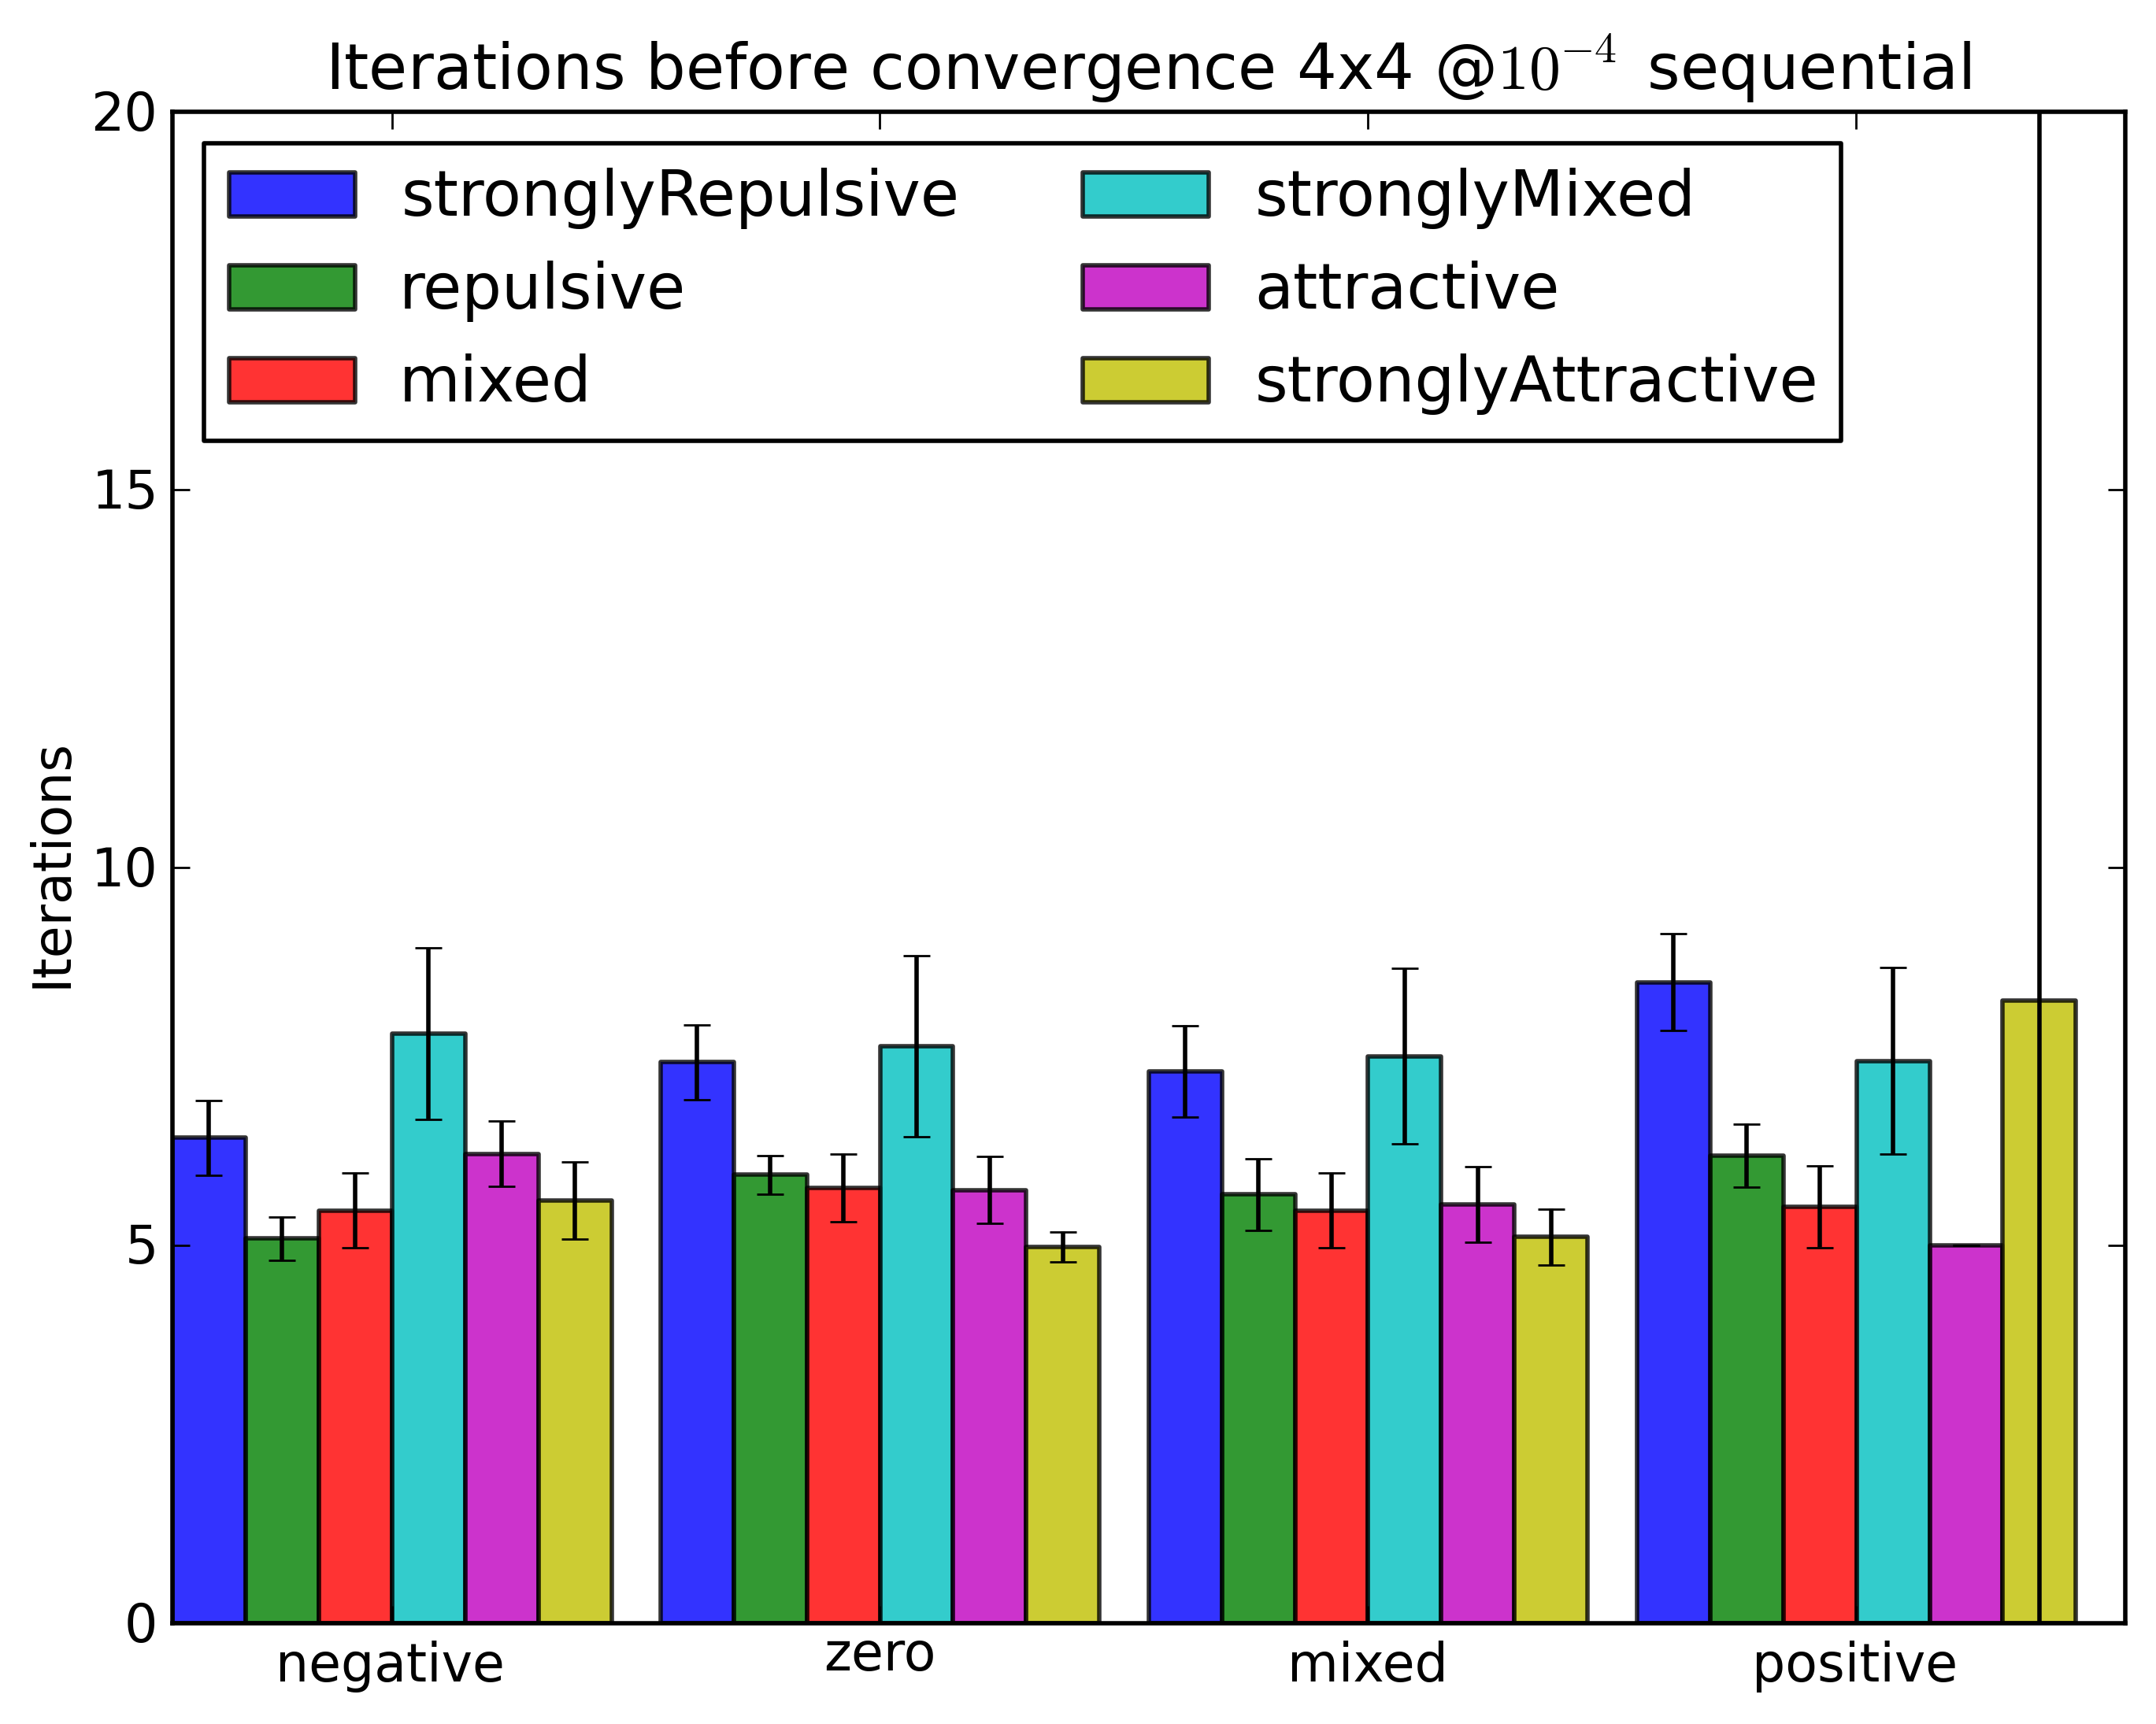
\includegraphics[width=9cm]{plots/convergence/iterations_before_convergence_4x4_e-4_sequential.png}}\subfigure[Naive parallel EP]{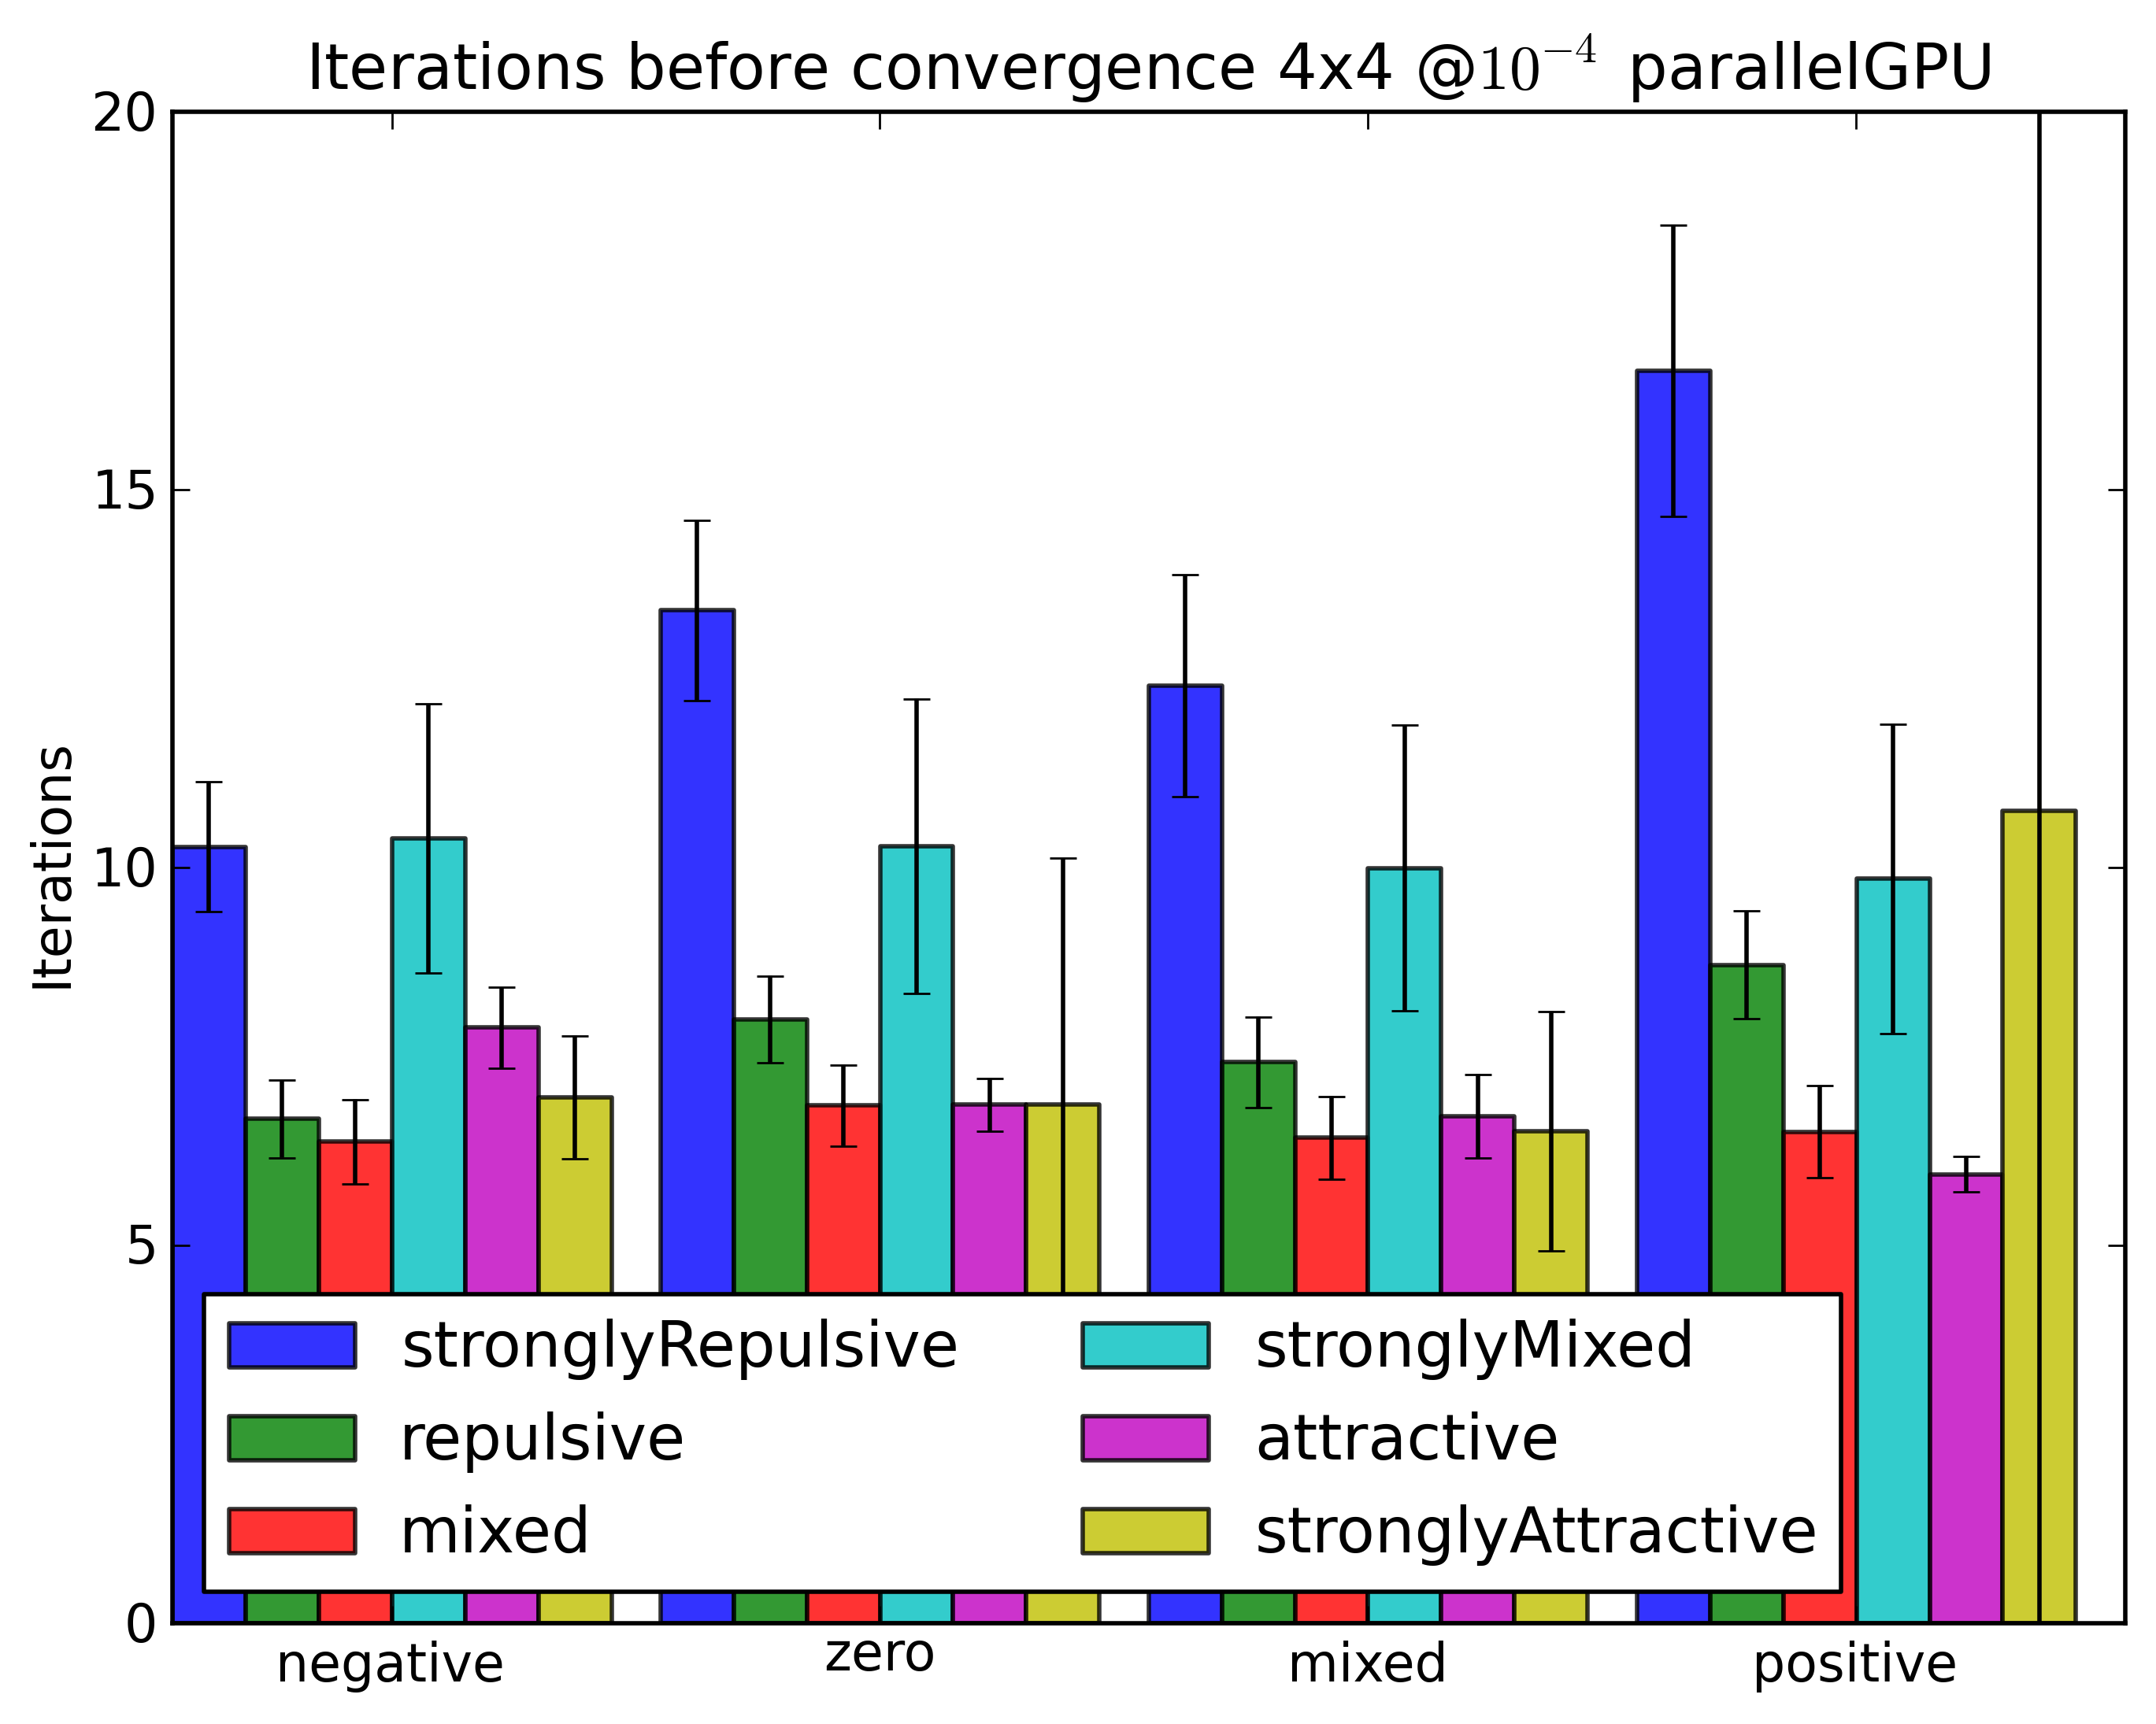
\includegraphics[width=9cm]{plots/convergence/iterations_before_convergence_4x4_e-4_parallelGPU.png}}
	\subfigure[Convexified EP]{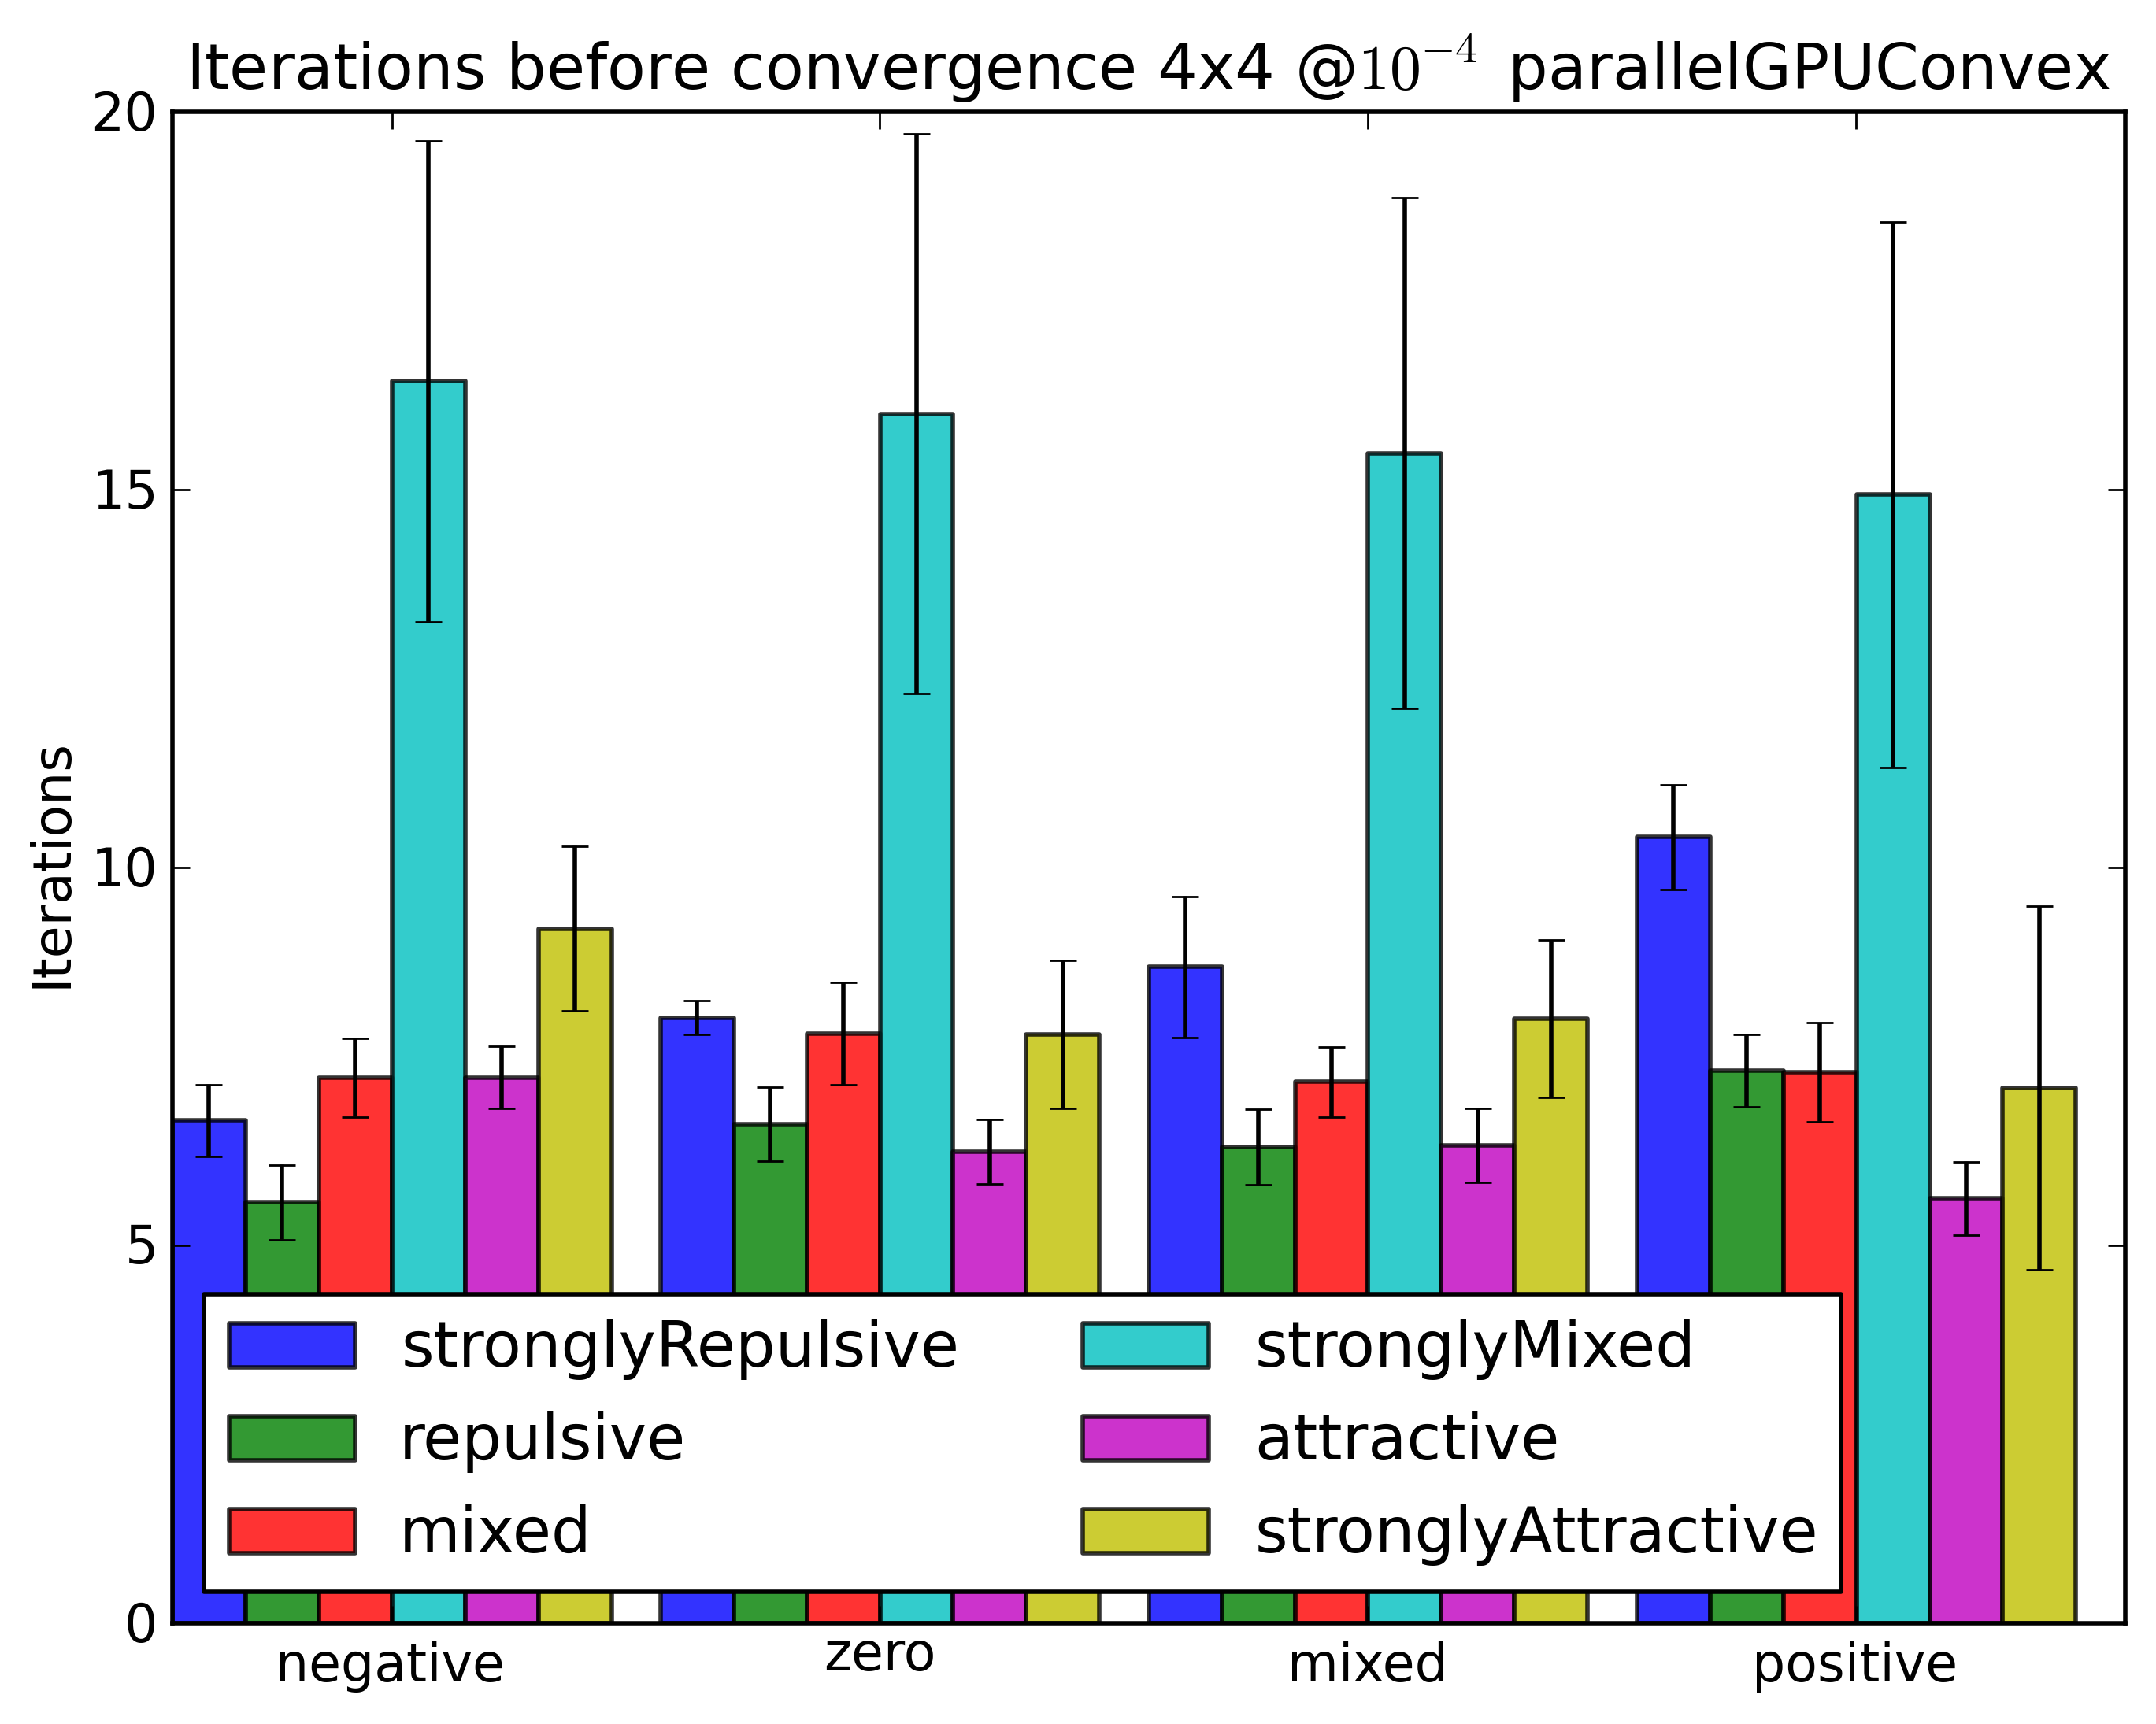
\includegraphics[width=9cm]{plots/convergence/iterations_before_convergence_4x4_e-4_parallelGPUConvex.png}}\subfigure[Pseudo-Convexified EP]{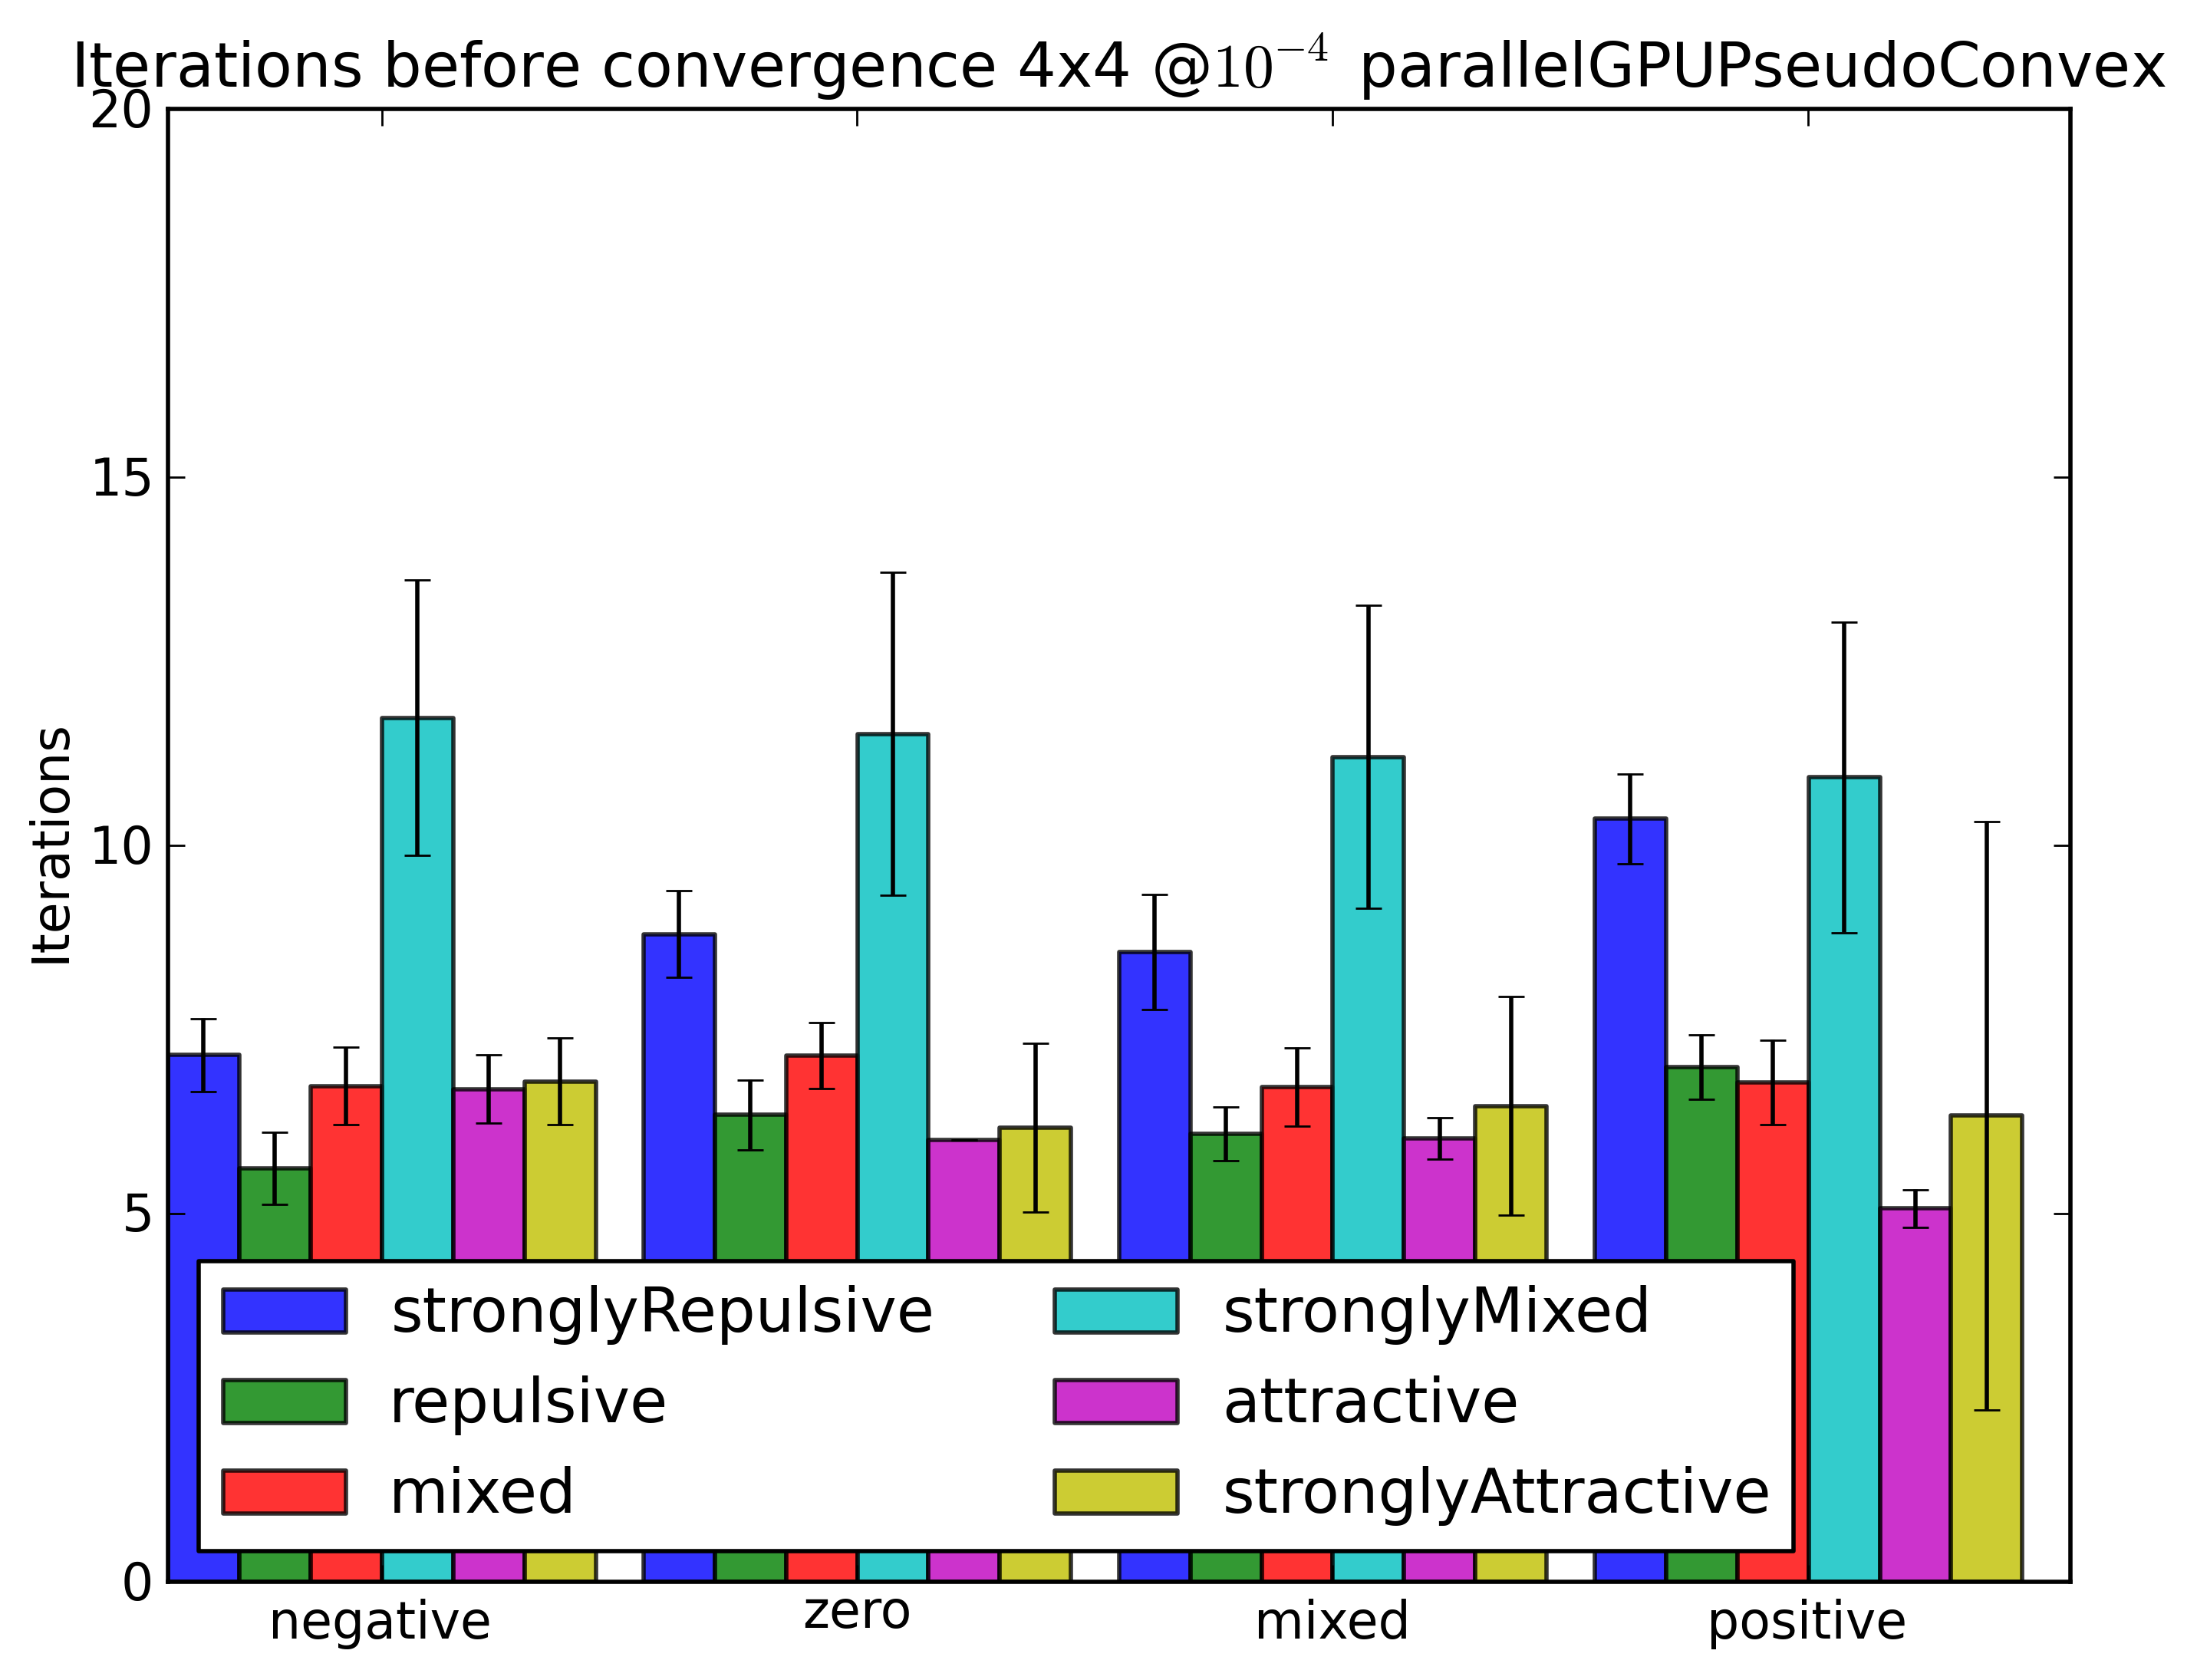
\includegraphics[width=9cm]{plots/convergence/iterations_before_convergence_4x4_e-4_parallelGPUPseudoConvex.png}}
	\caption{Number of iterations before computed marginals change less than $10^{-4}$ in relative $L_1$ norm. Results are averaged over 100 $4 \times 4$ Ising instances per Ising type. Error bars are shown at 1 sigma. Notice that both the sequential and the naive parallel version of EP do not converge on some instances of positive strongly attractive models, but that the convex and pseudo-convex algorithms always converge.}
\end{figure}

\newpage

\begin{figure}\centering
	\subfigure[Sequential EP]{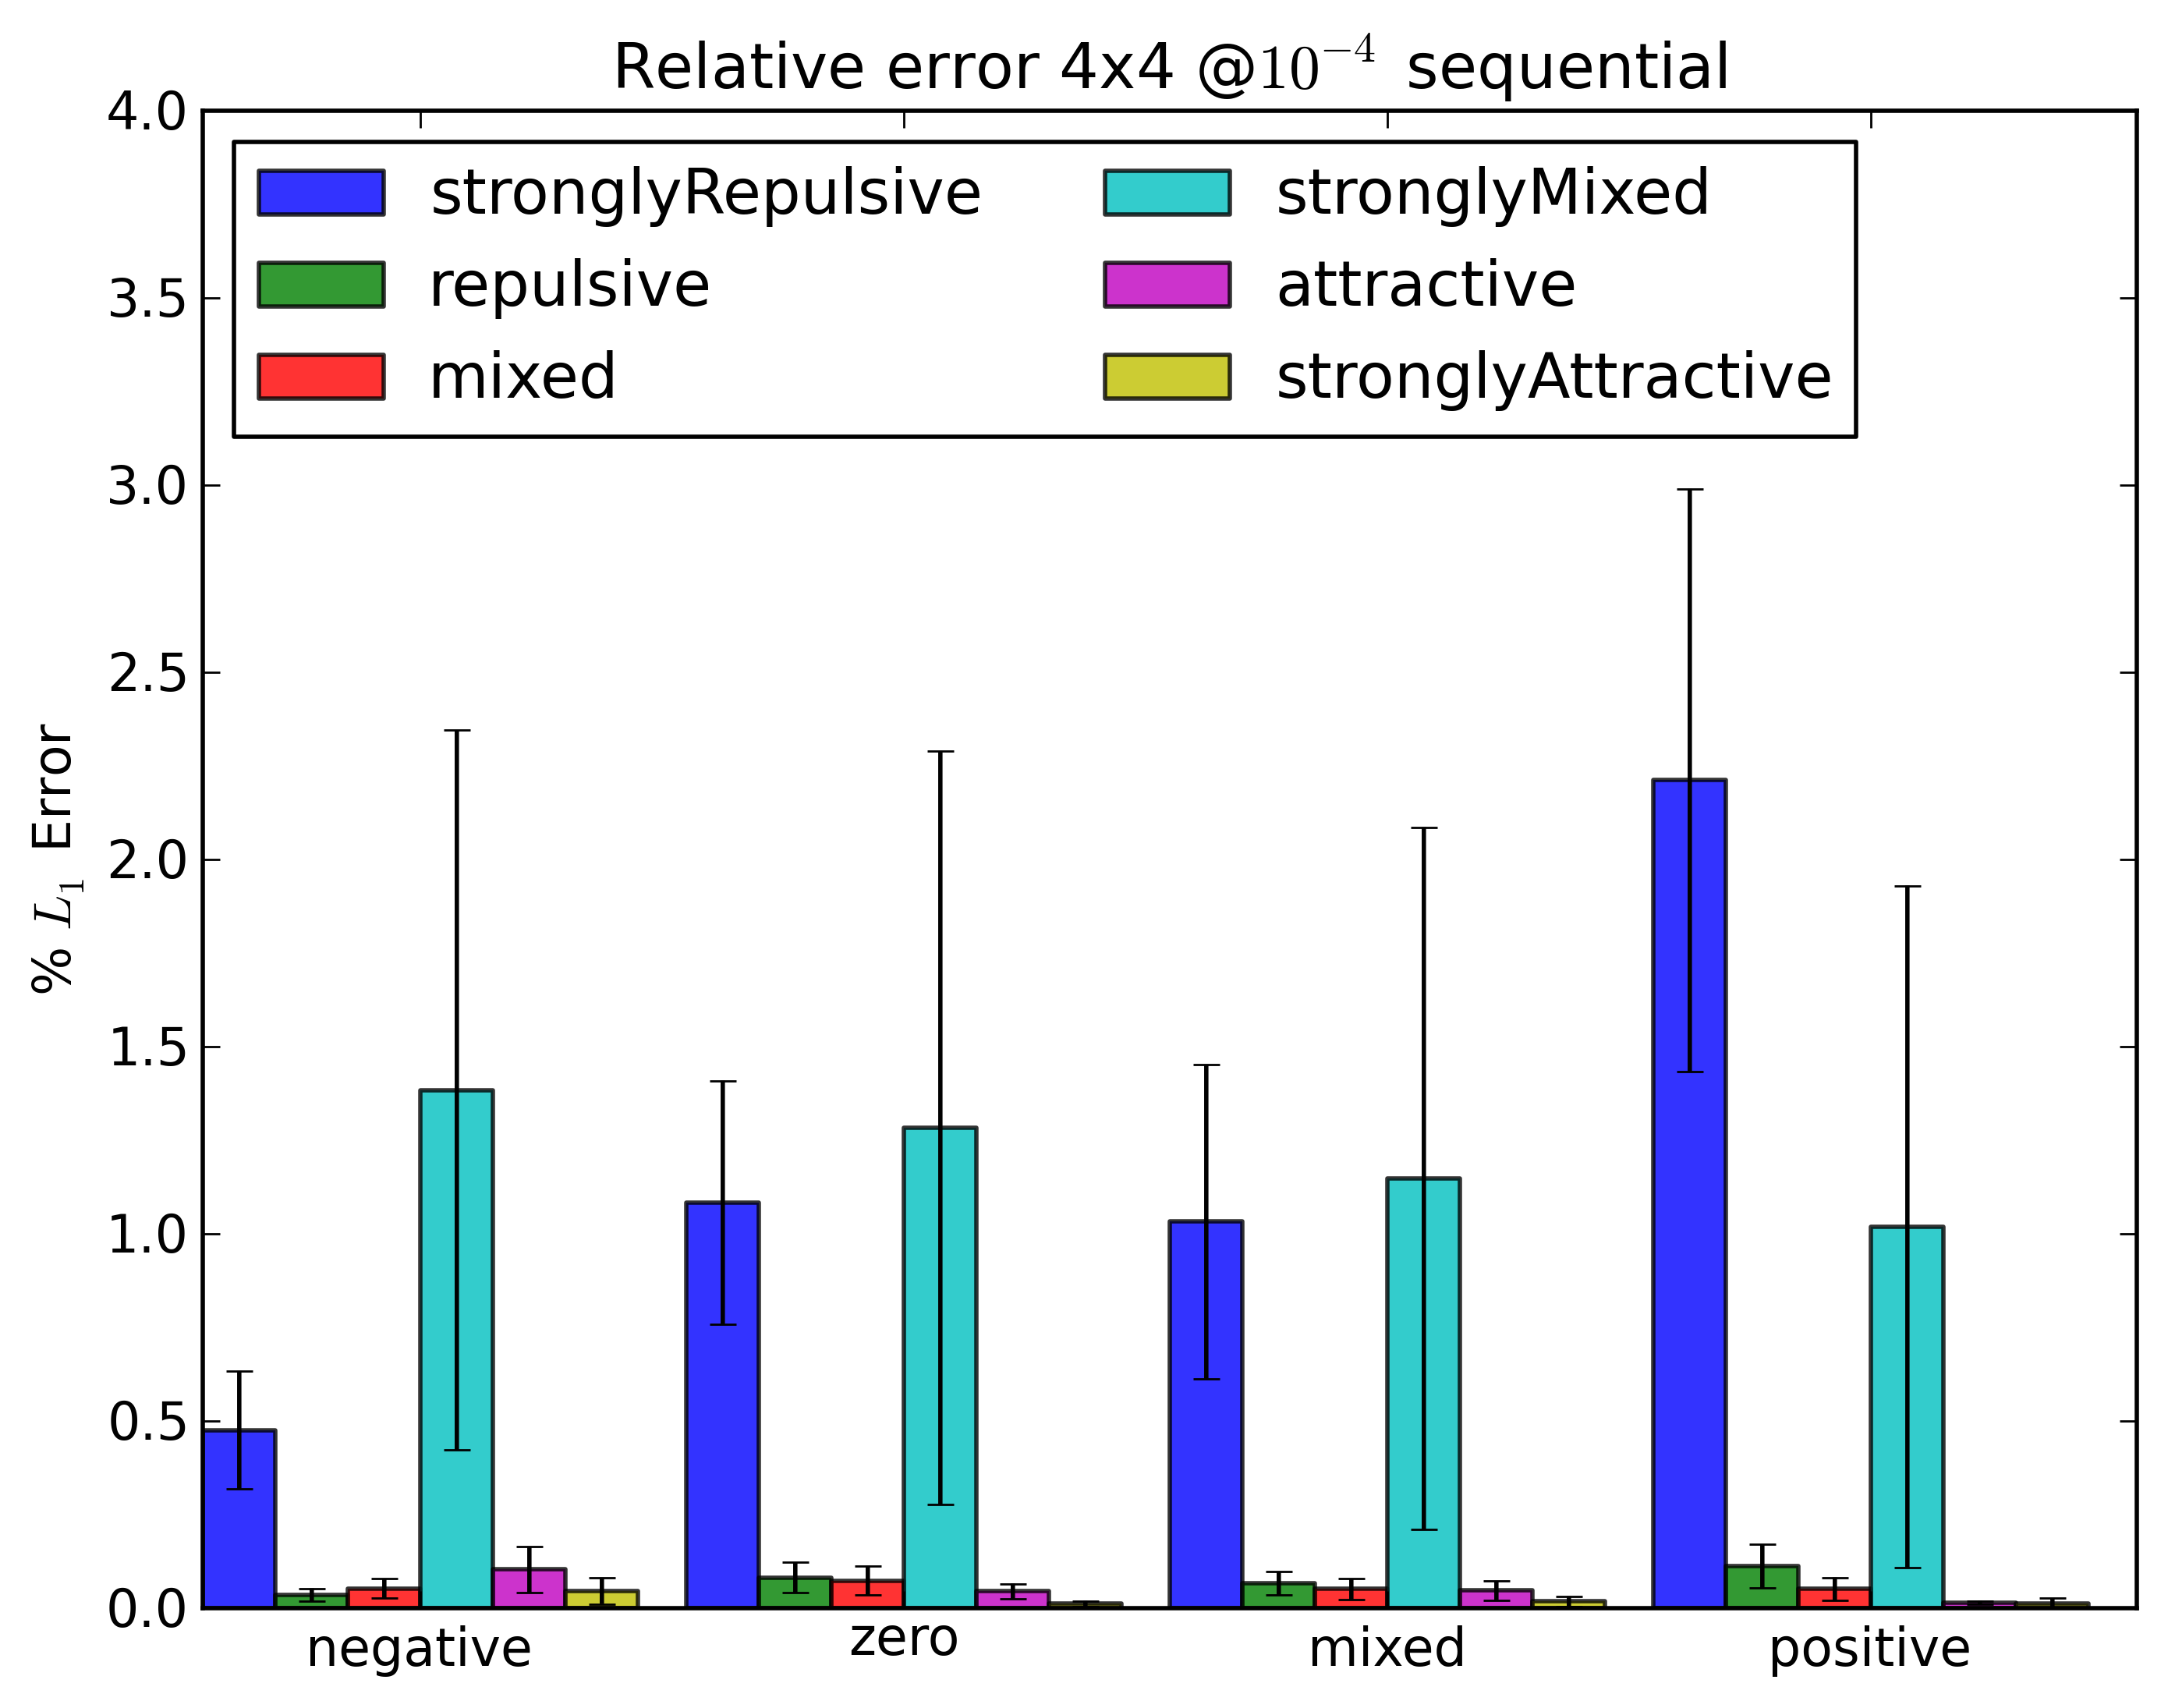
\includegraphics[width=9cm]{plots/accuracy/Relative_error_4x4_e-4_sequential.png}}\subfigure[Naive parallel EP]{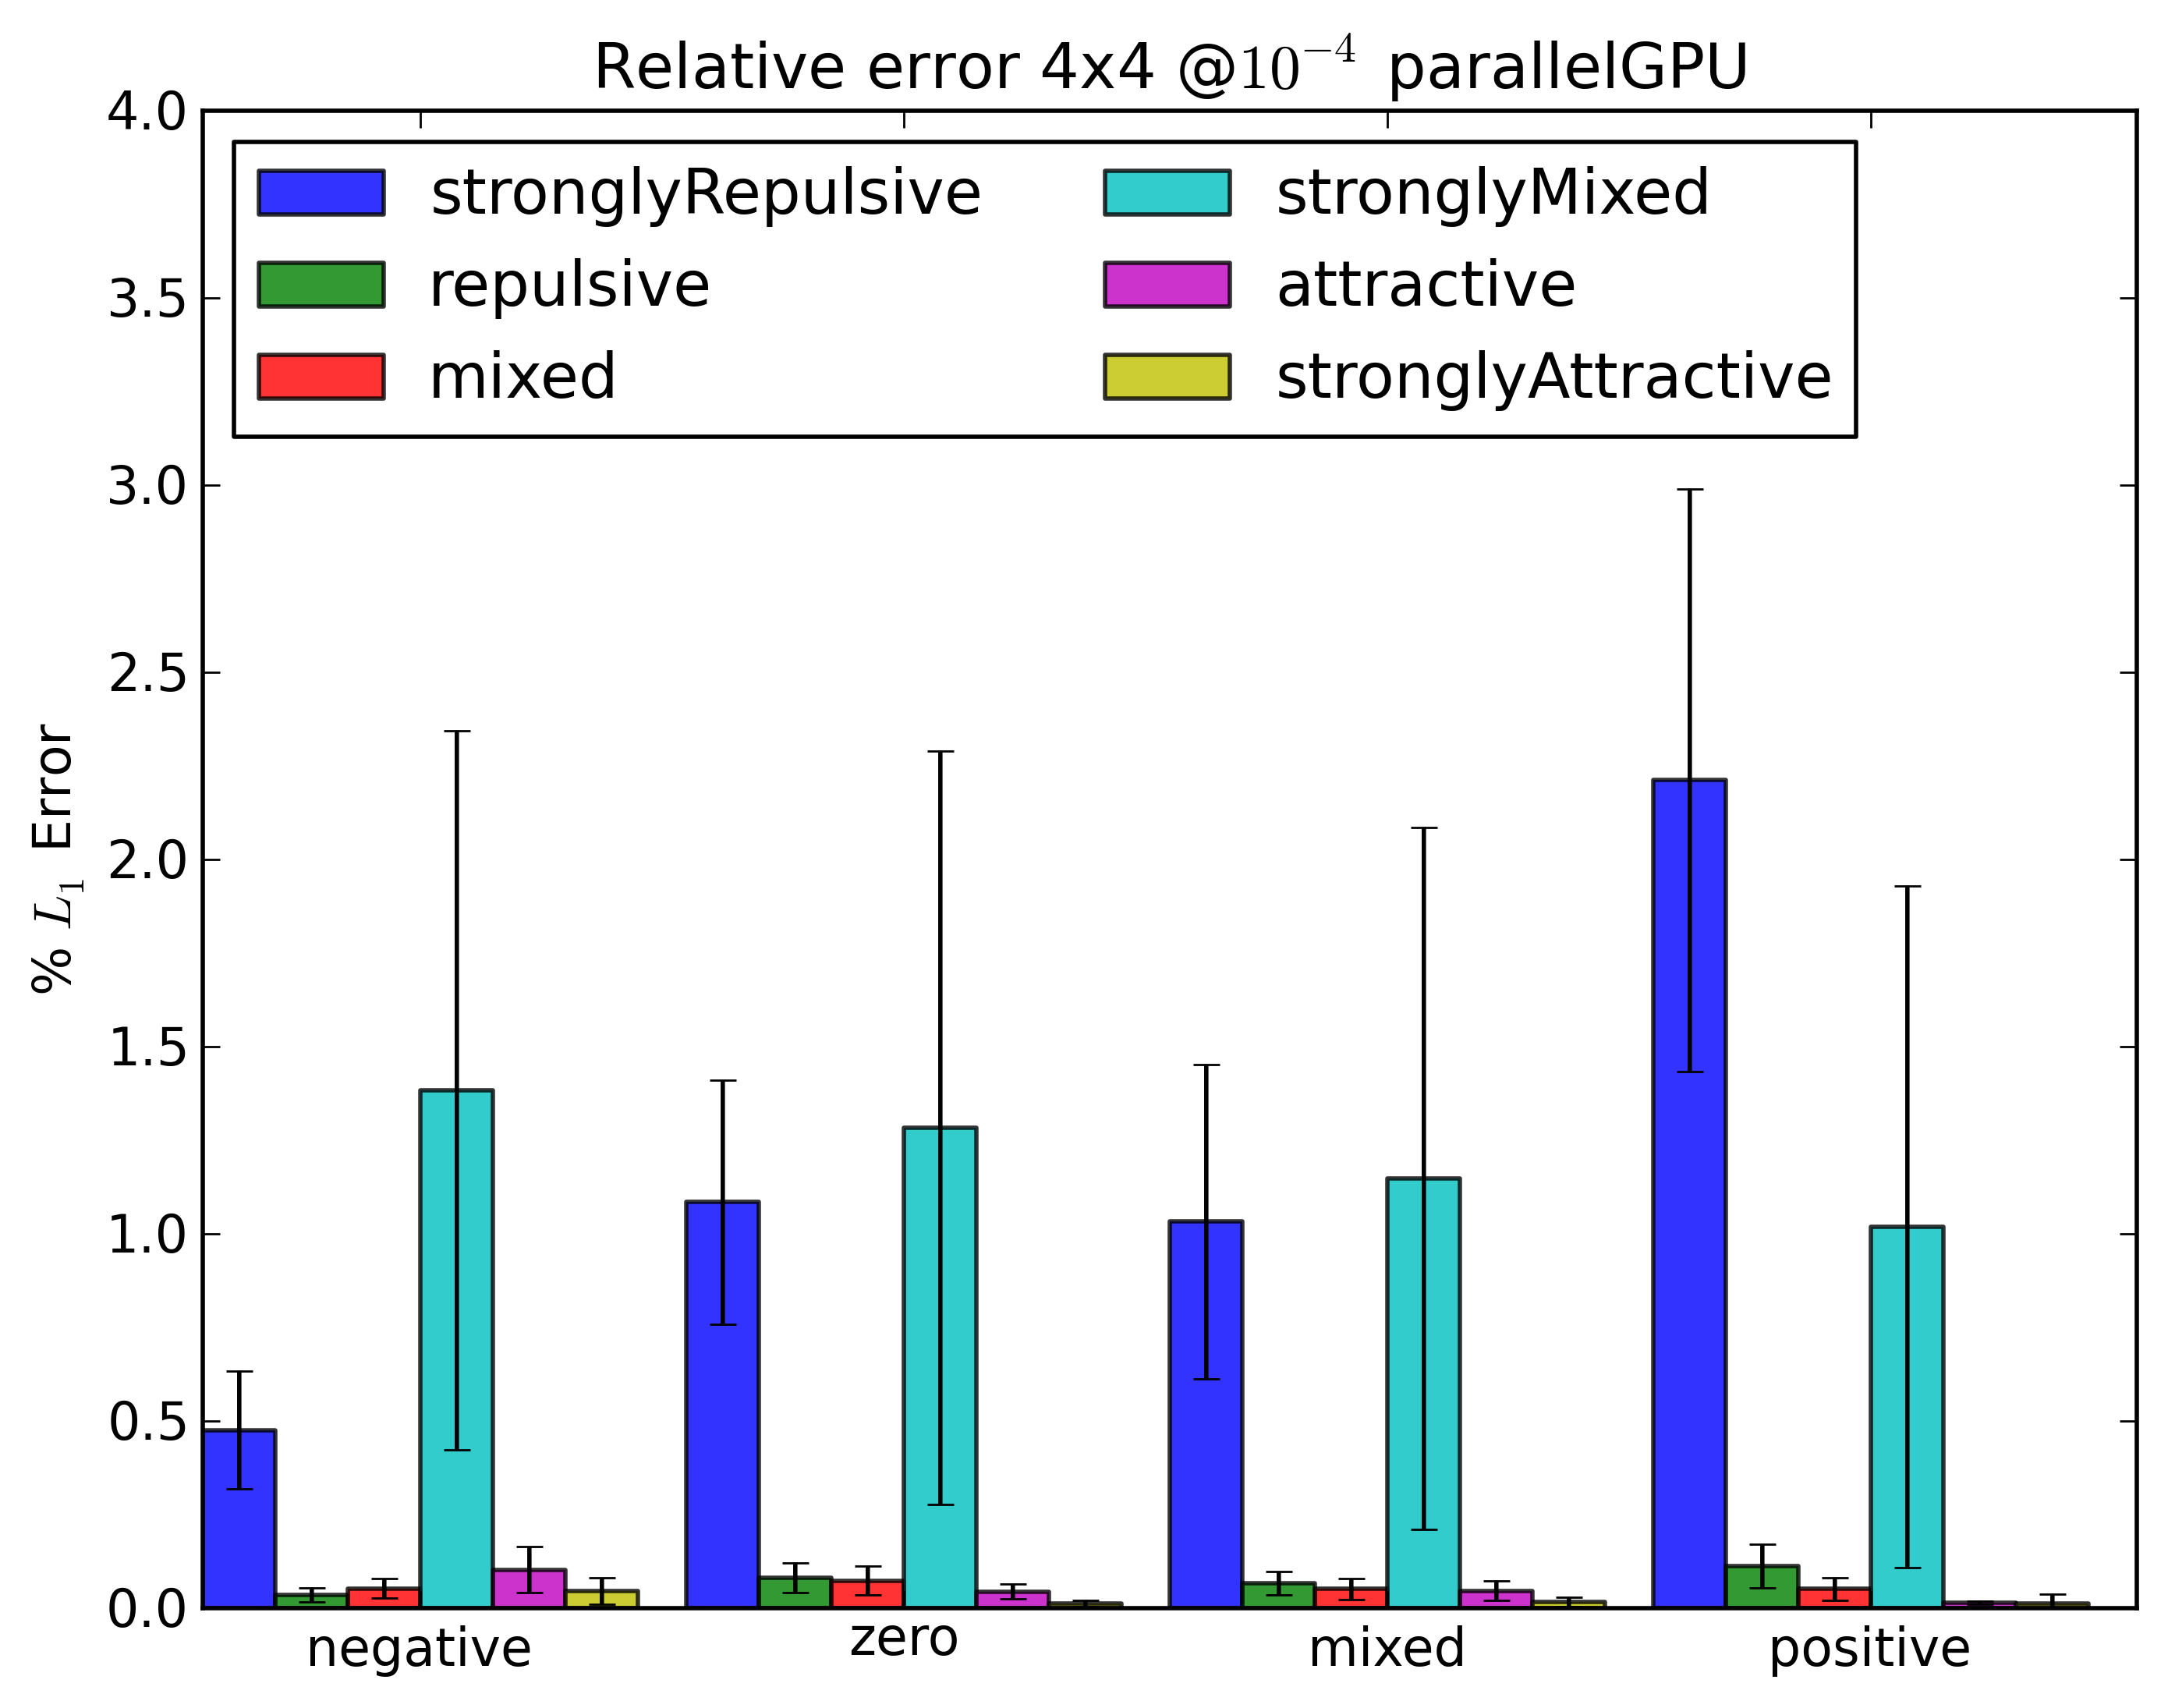
\includegraphics[width=9cm]{plots/accuracy/Relative_error_4x4_e-4_parallelGPU.png}}
	\subfigure[Convexified EP]{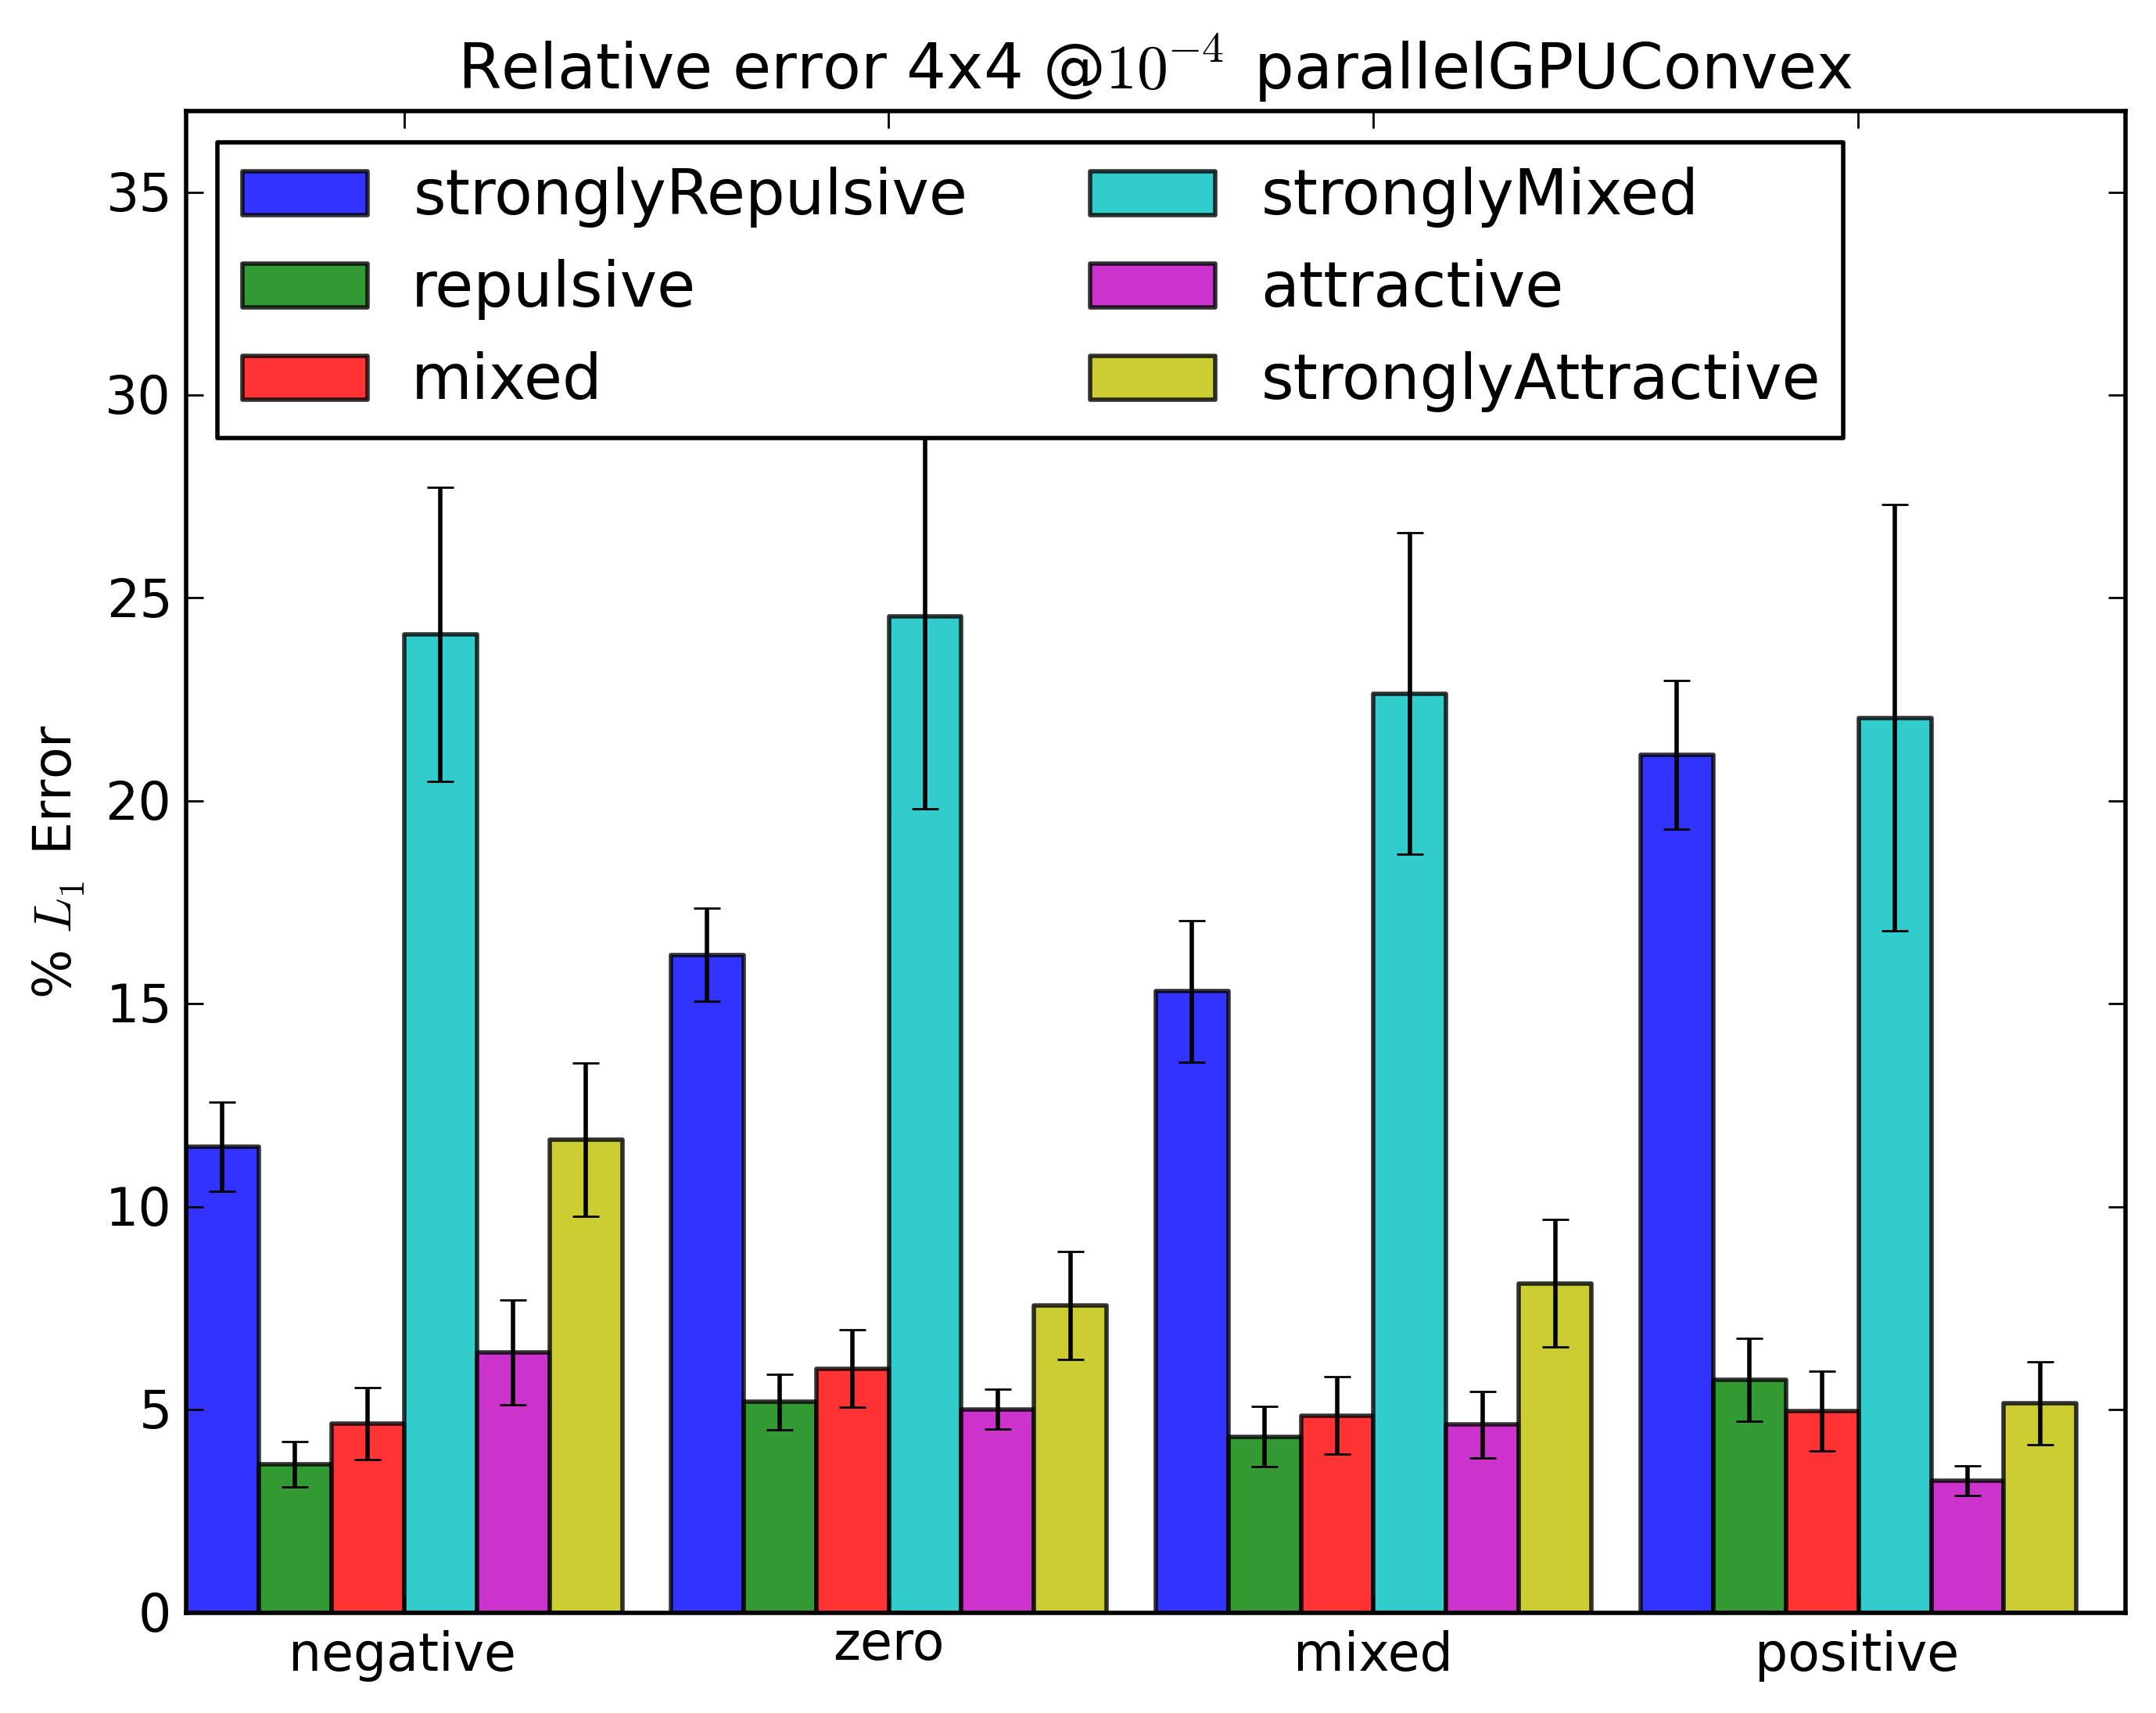
\includegraphics[width=9cm]{plots/accuracy/Relative_error_4x4_e-4_parallelGPUConvex.png}}\subfigure[Pseudo-Convexified EP]{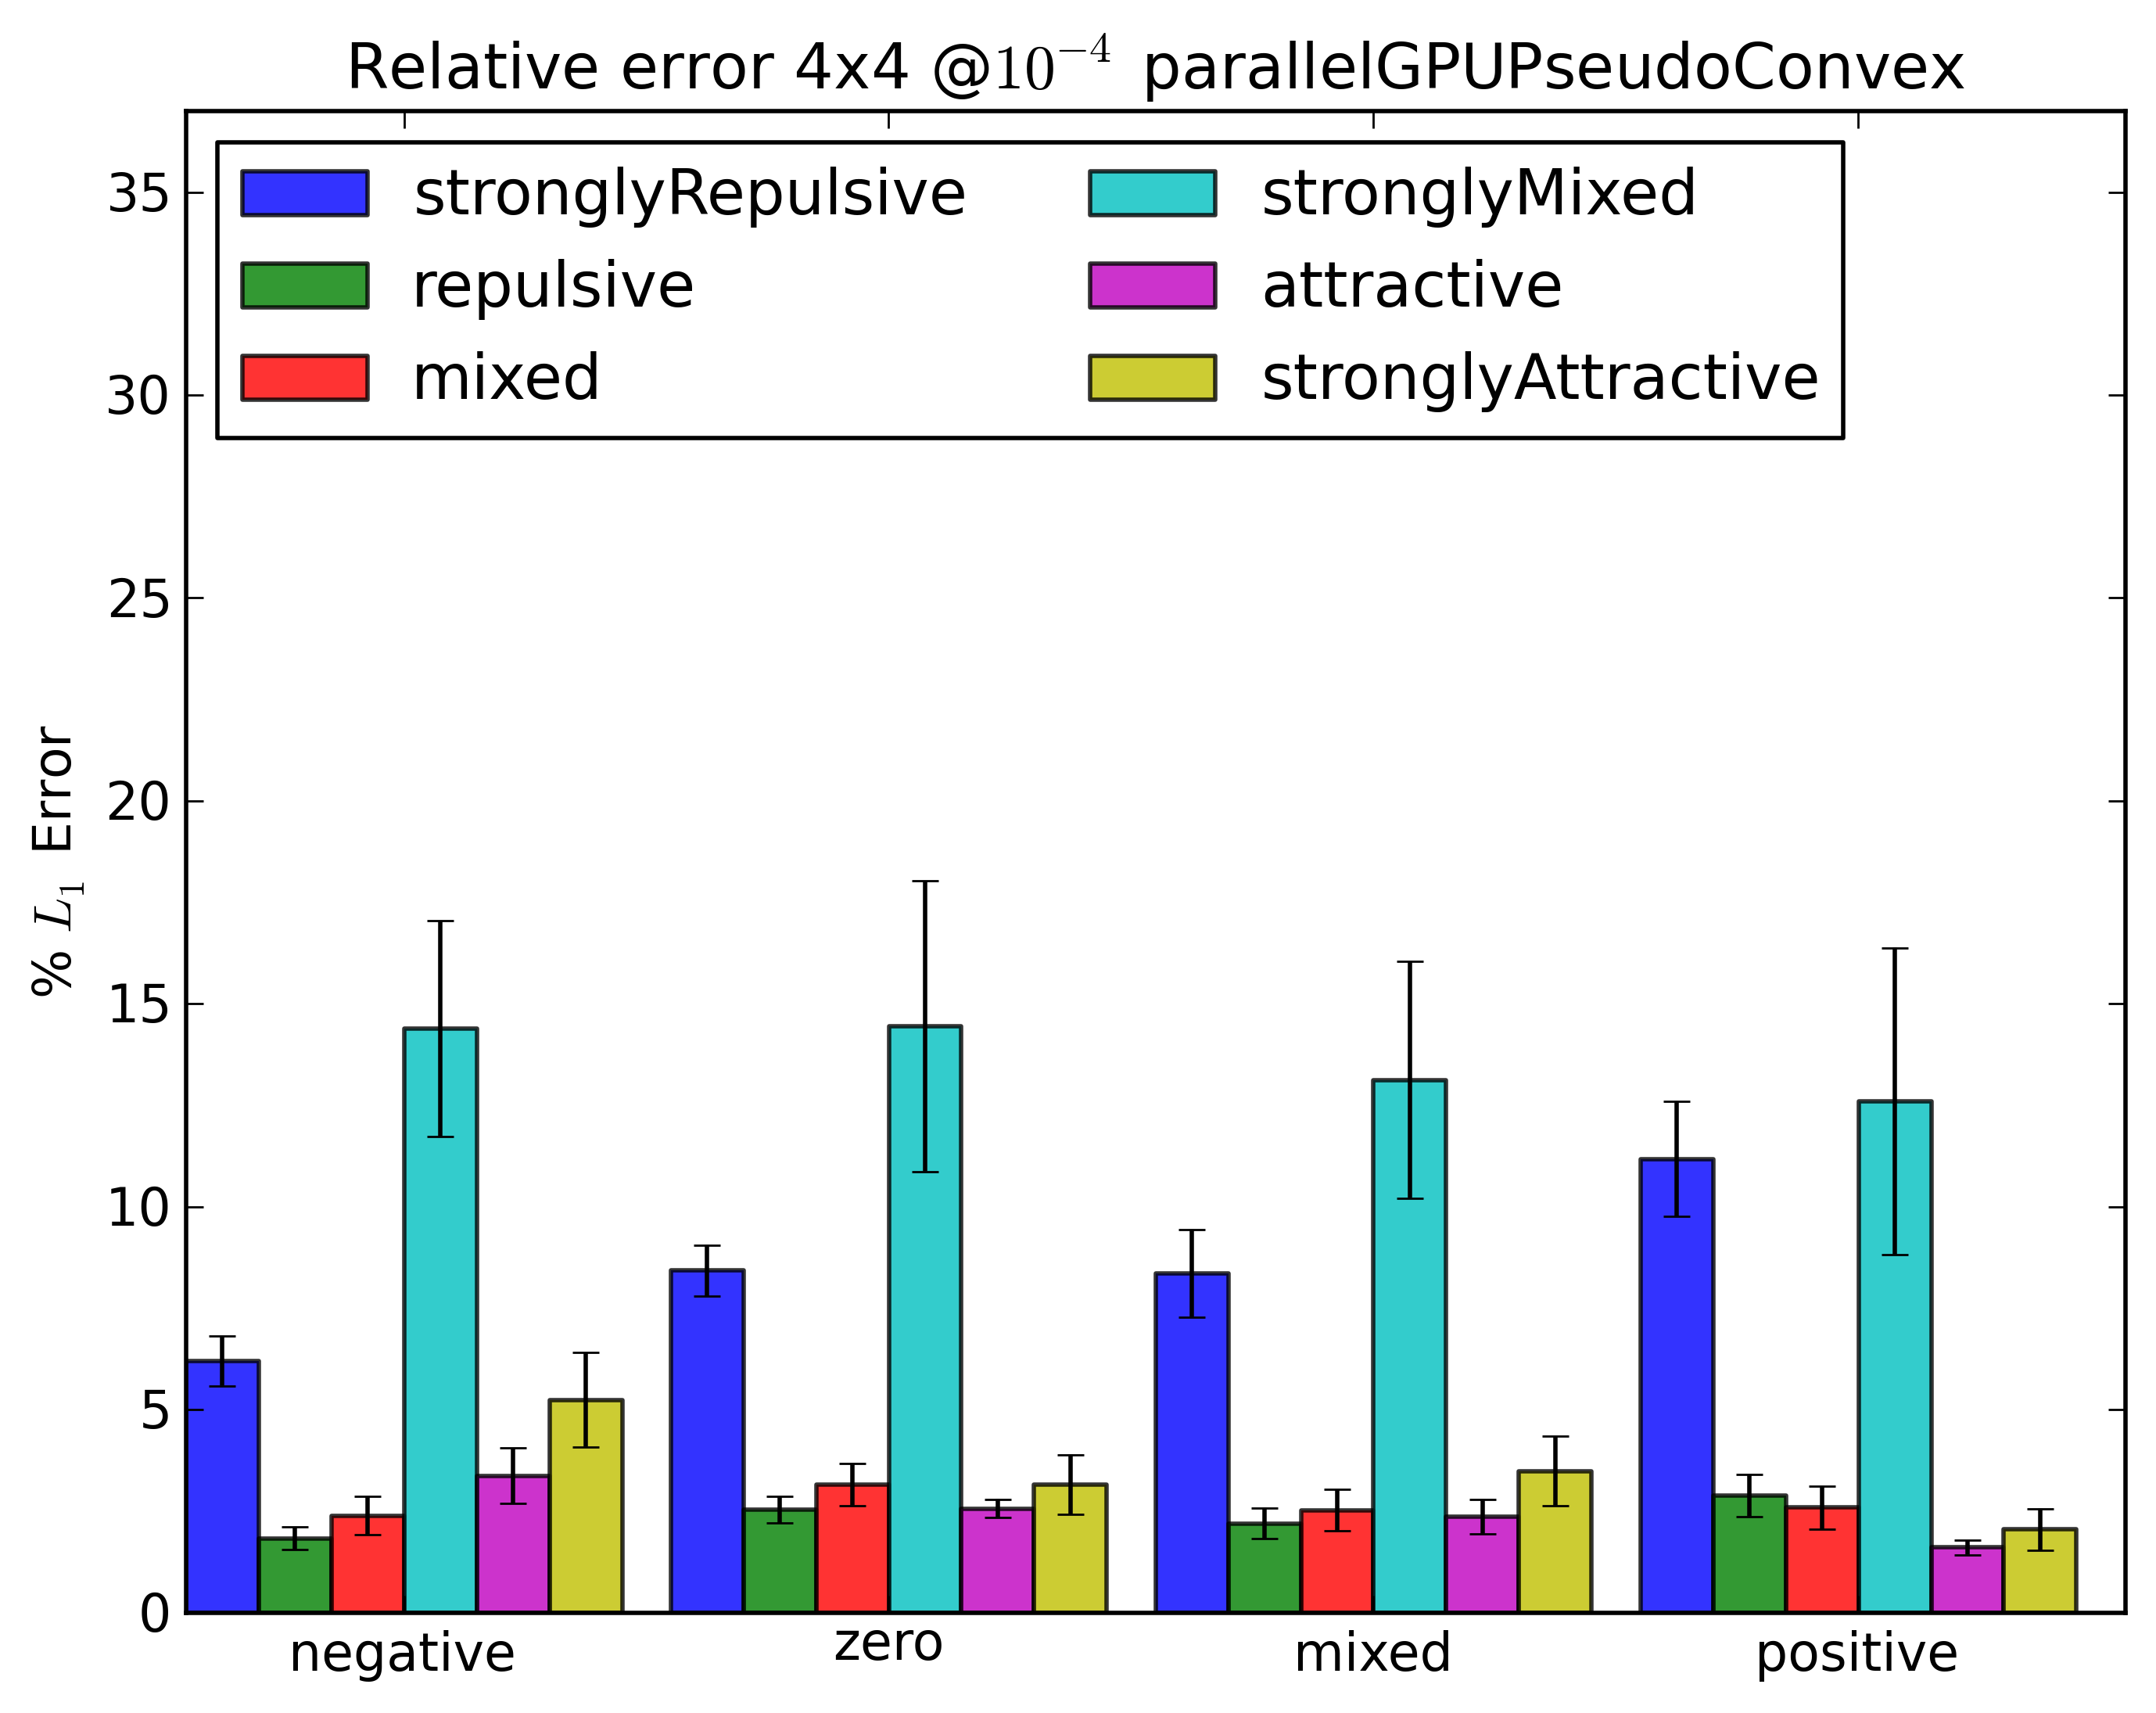
\includegraphics[width=9cm]{plots/accuracy/Relative_error_4x4_e-4_parallelGPUPseudoConvex.png}}
	\caption{Relative $L_1$ error after $10^{-4}$ convergence. Results are averaged over 100 $4 \times 4$ Ising instances per Ising type. Error bars are shown at 1 sigma. For this size of models, there is no significant difference in accuracy between sequential EP and naive parallel EP. Convex EP and pseudo-convex EP both show significant accuracy degradation with respect to EP.}
\end{figure}

\newpage
\subsection{Increasing model size}
Interesting instances with respect to convergence are the negative strongly mixed, positive strongly repulsive and strongly attractive. We will only focus on these family instances.

\newpage
\begin{figure}\centering
	\subfigure[Convergence]{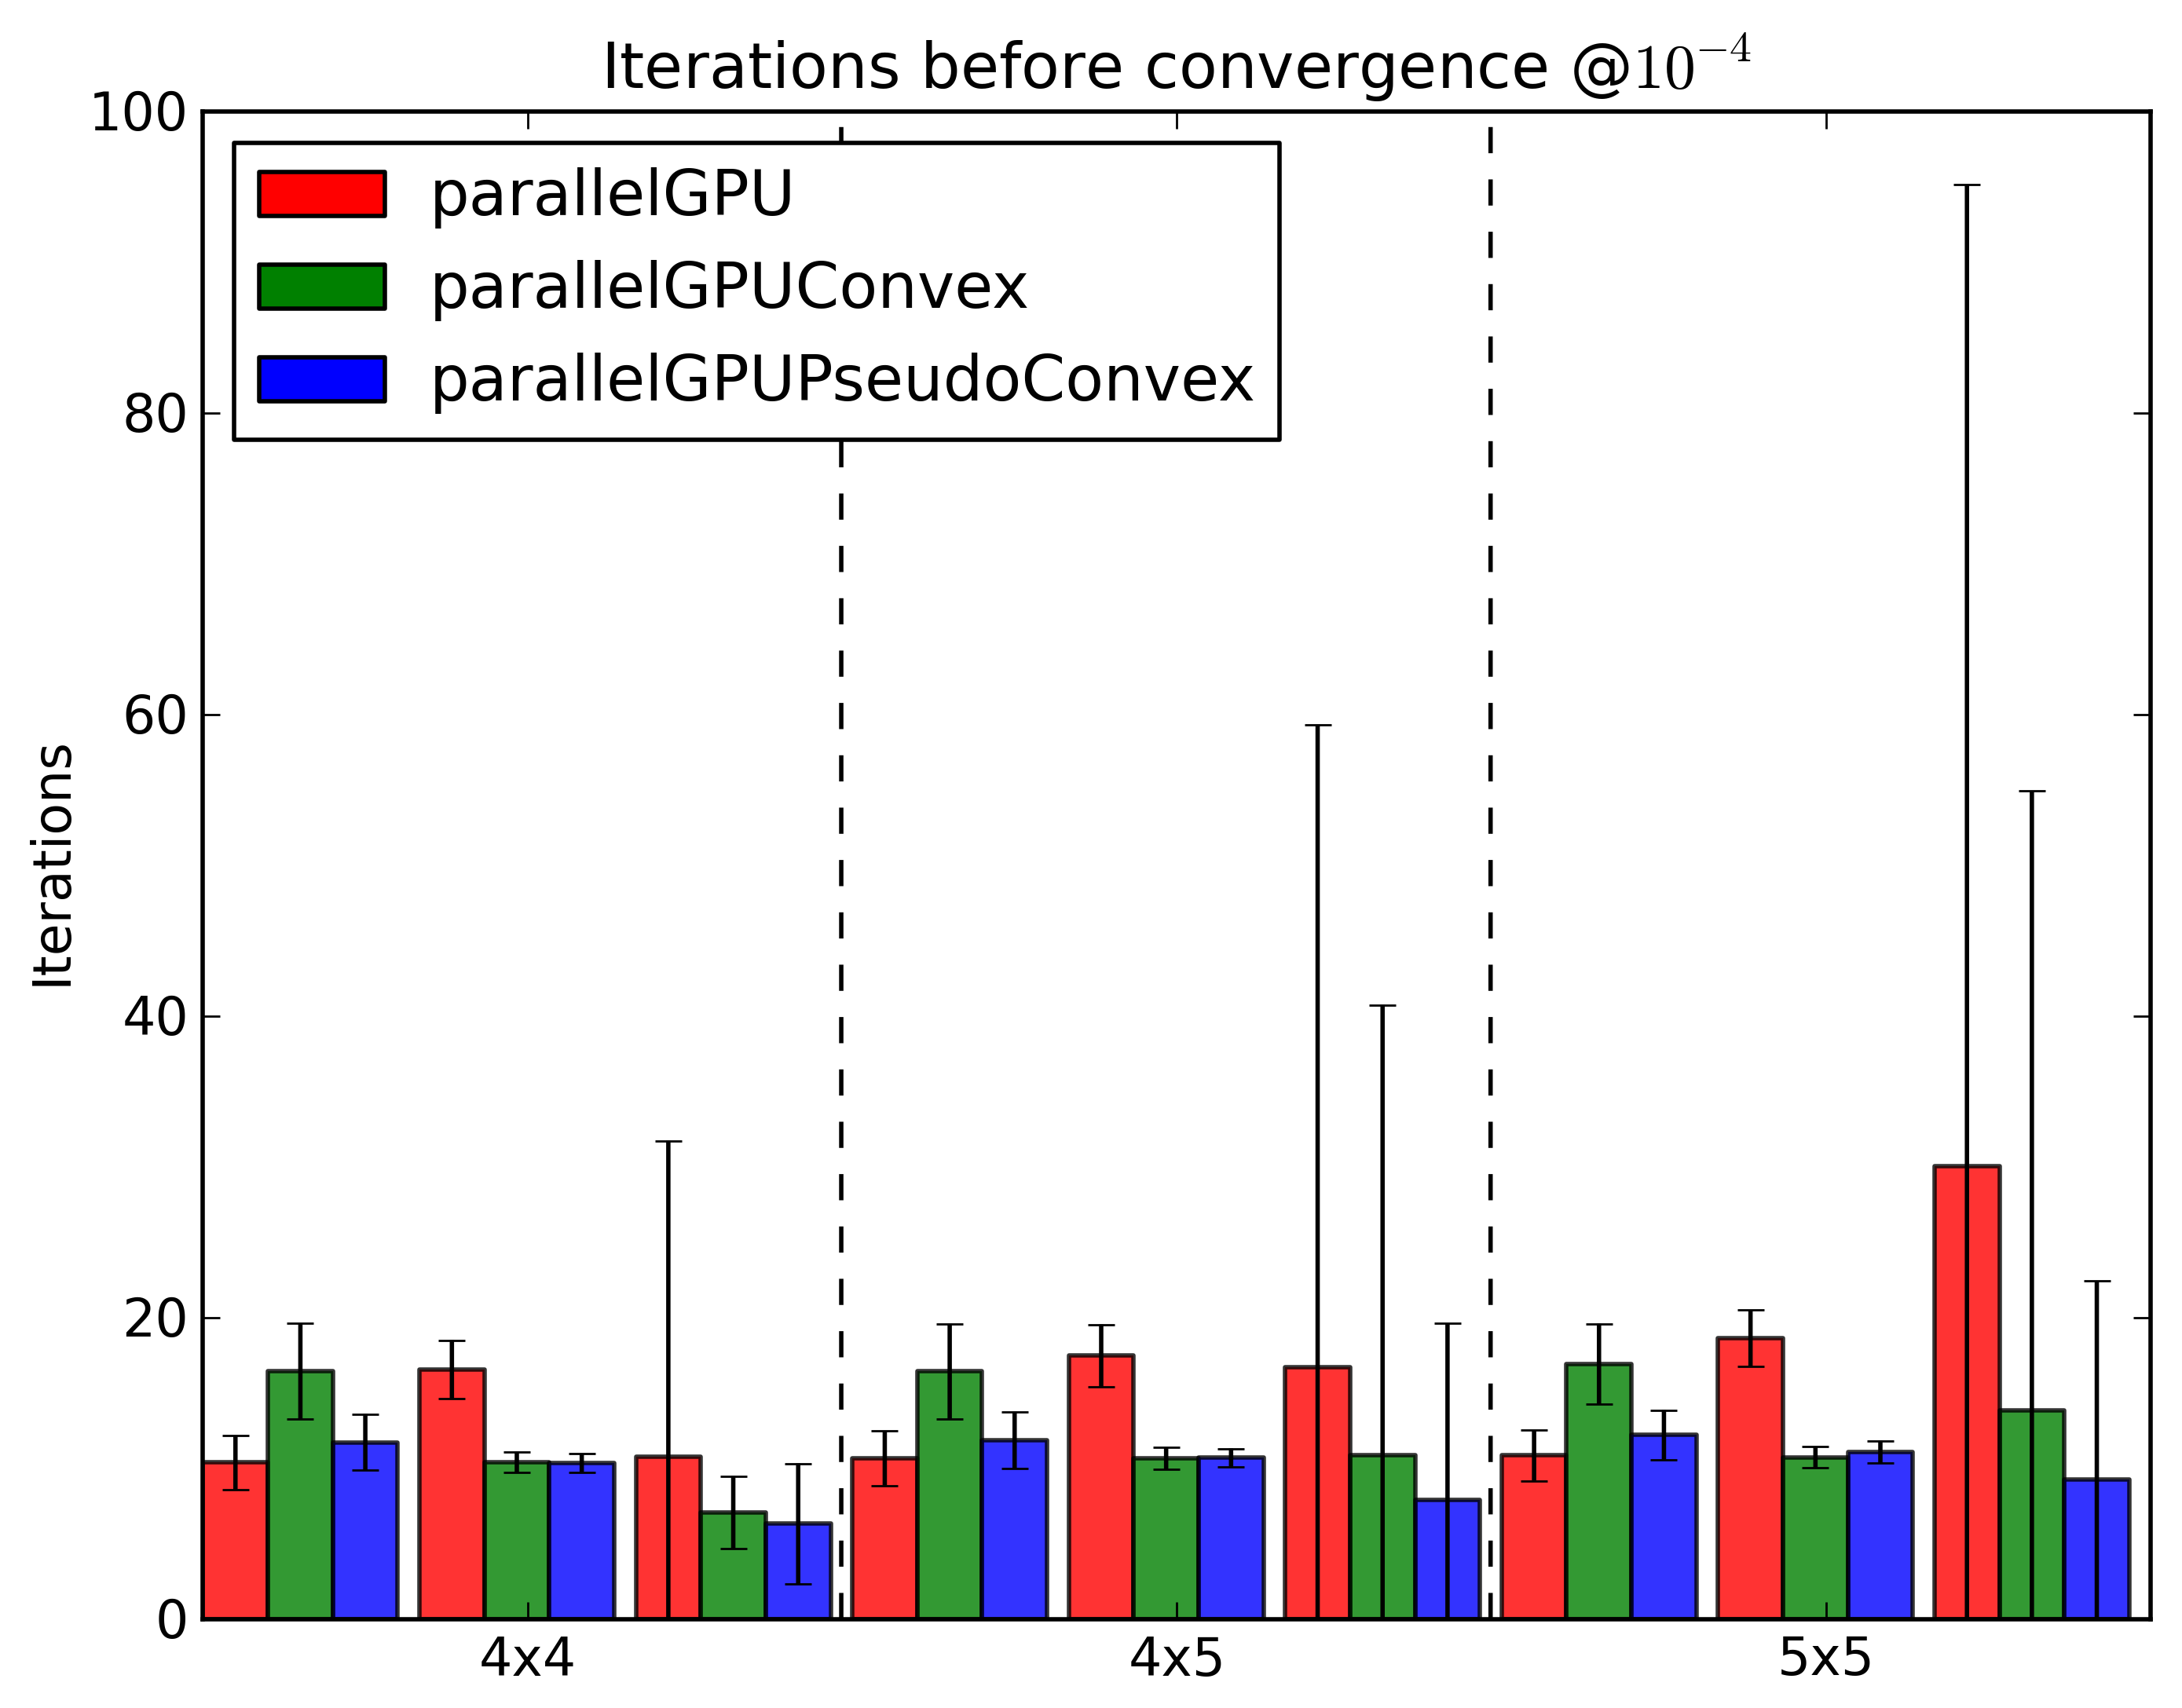
\includegraphics[width=8cm]{plots/sizes/iterations_before_convergence_e-4.png}}
	\subfigure[Accuracy]{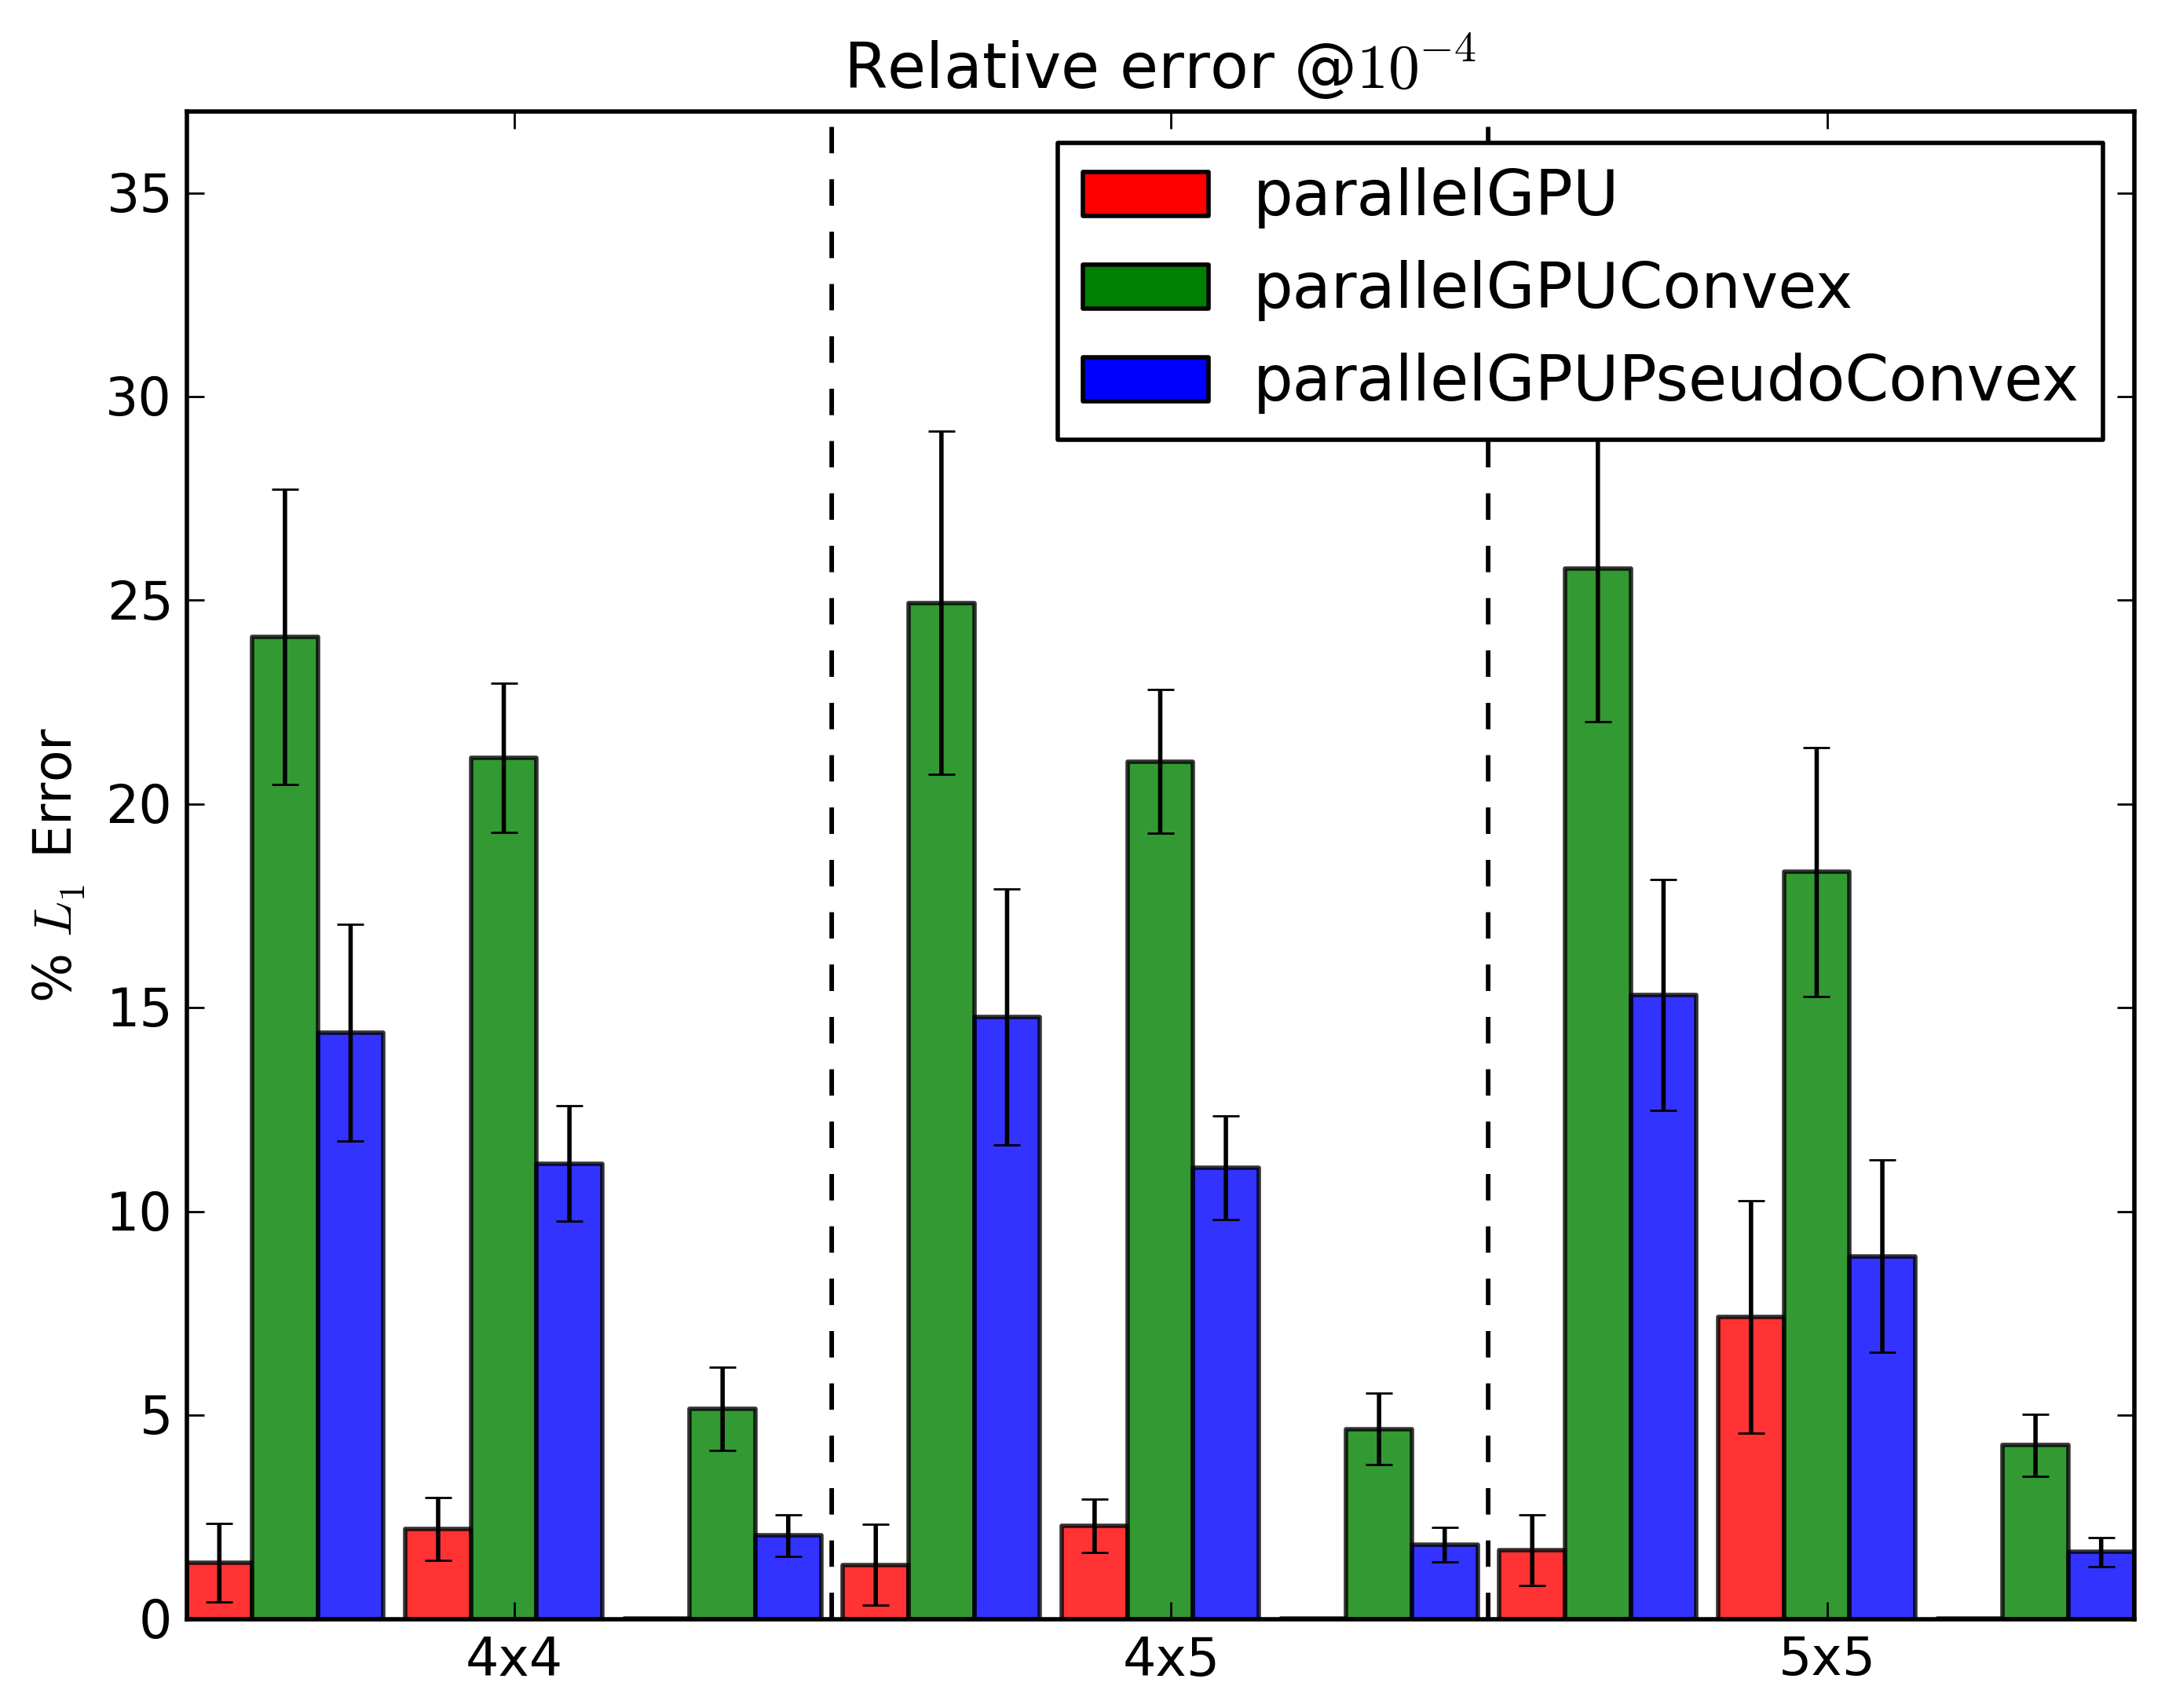
\includegraphics[width=8cm]{plots/sizes/relative_error_e-4.png}}
	\caption{Convergence and accuracy measures over $4 \times 4$, $4 \times 5$ and $5 \times 5$ models. Each group of 3 bars within a given instance size respectively represent negative strongly mixed, positive strongly repulsive and positive strongly attractive instances. The convexified and pseudo-convexified EP versions do improve convergence at a significant cost in terms of accuracy with respect to the naive parallel EP.}
\end{figure}

\begin{figure}\centering
	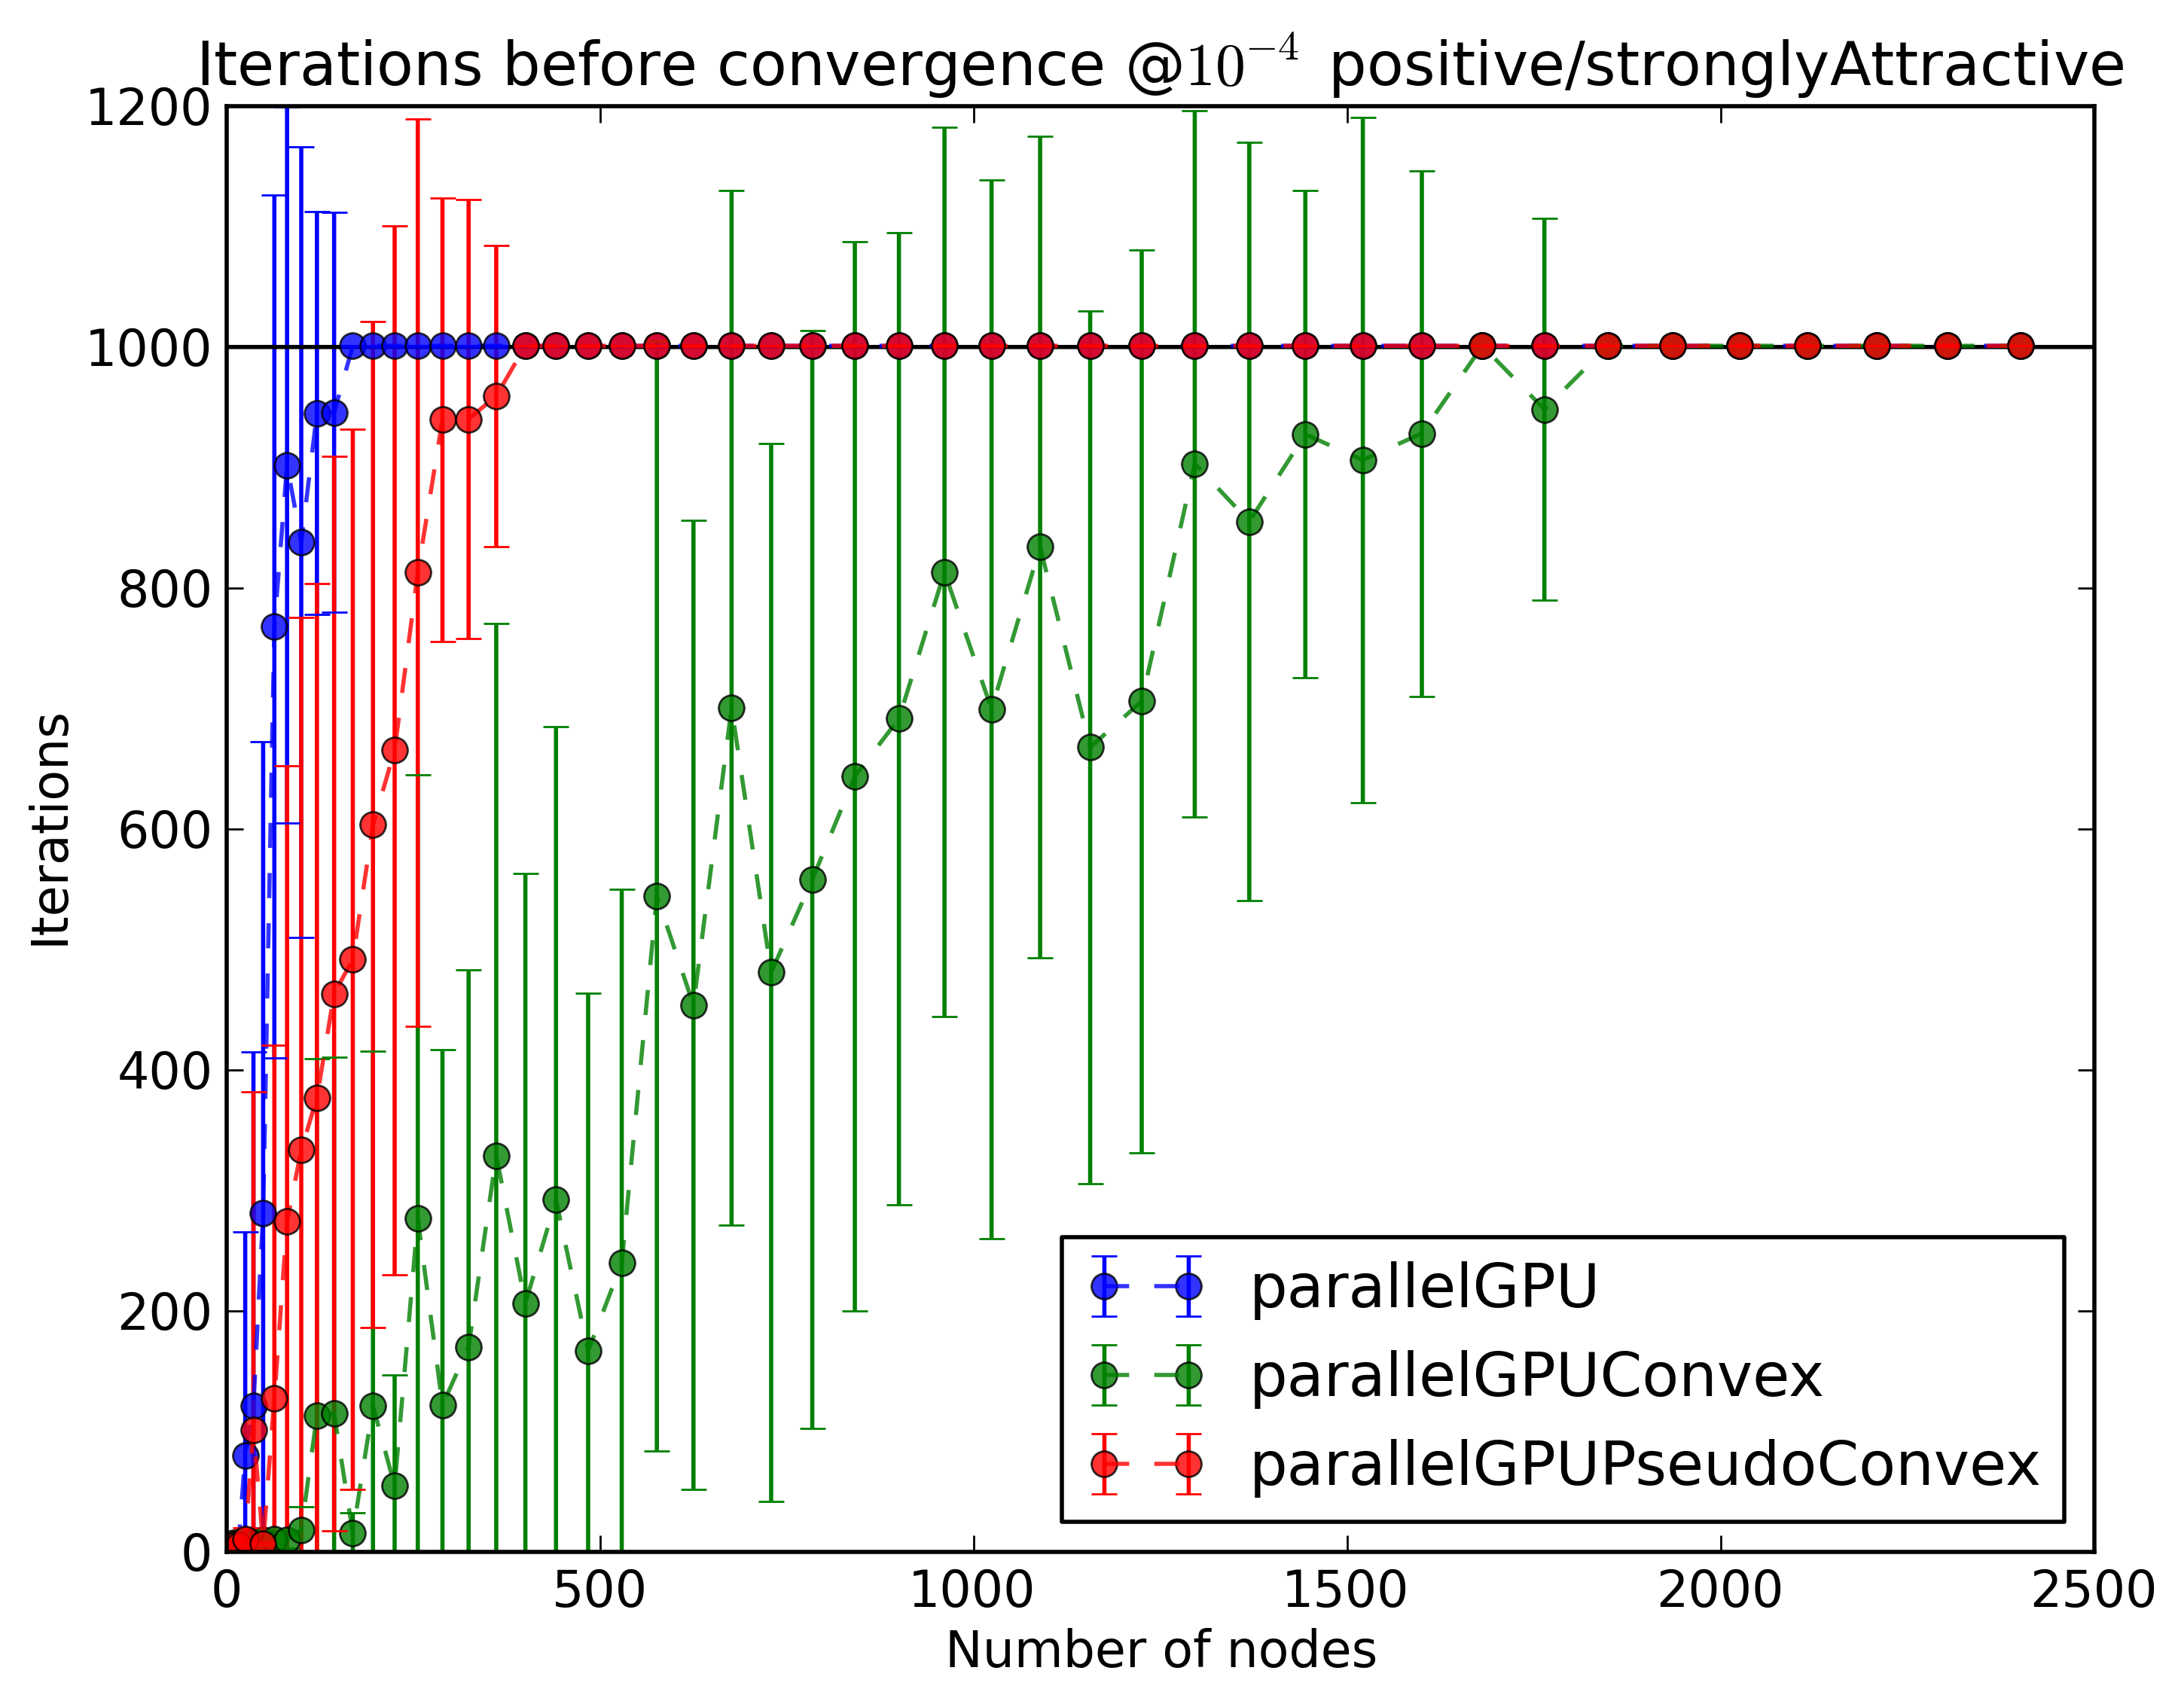
\includegraphics[width=8cm]{plots/sizes/Iterations_before_convergence_e-4_positive_stronglyAttractive.png}
	\caption{Eventually, both convex and pseudo-convex EP diverge on large positive strongly attractive instances. The maximum number of iterations was set to 1000 in this measurement.}
\end{figure}

\begin{figure}\centering
	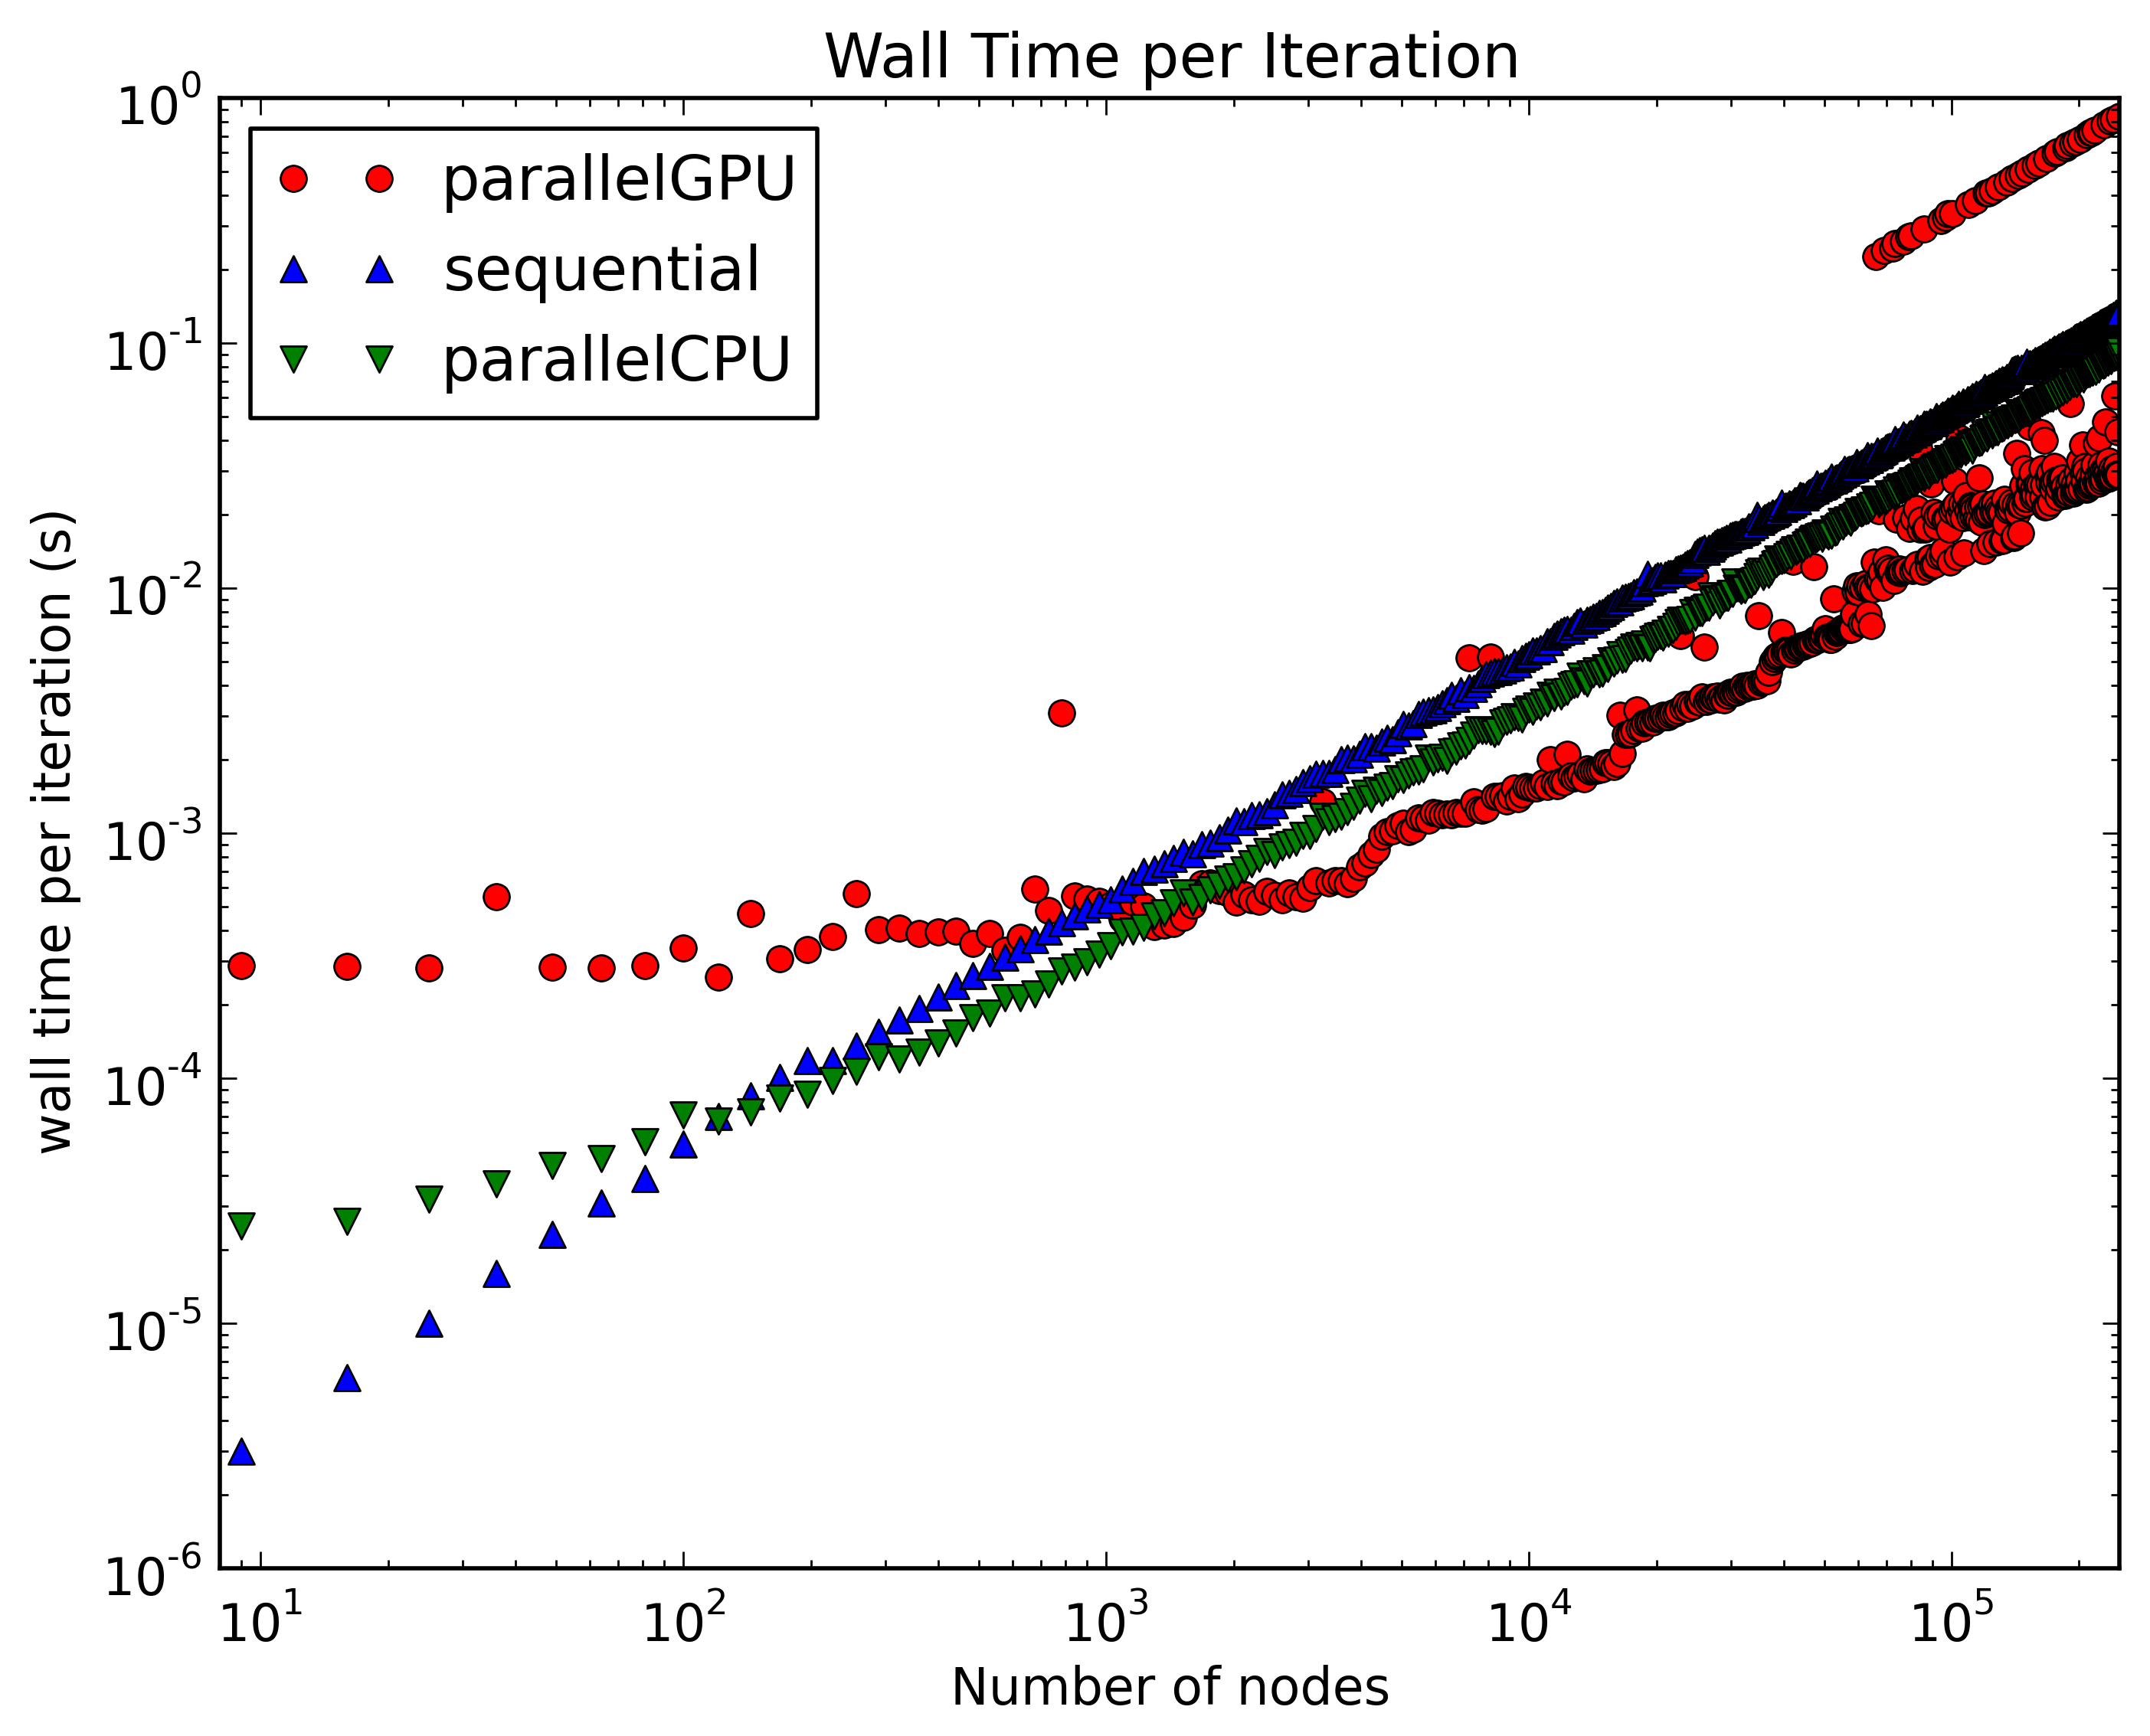
\includegraphics[width=8cm]{plots/sizes/time_per_iteration.png}
	\caption{Log-log plot of the wall time per iteration of sequential EP and parallel EPs (naive, convex and pseudo-convex) ran on a 4 cores Intel i7 CPU and a low end laptop GPU (AMD Radeon HD 6490M). Asymptotic slopes are unitary as the algorithm is linear in the number of nodes. The bi-modal behavior of the GPU implementation for large instances is most probably due to the limited amount of on-chip memory available (256Mb). As for the smaller instances, we suspect some interference between the OS and the GPU, such as GUI rendering.}
\end{figure}


\section{Conclusion}


\nocite{ex1,ex2}
\bibliographystyle{latex8}
\bibliography{latex8}

\end{document}


